% Self-contained research-development manuscript.
% Build: pdflatex Machine_Markets_Concise_Final_Integrated_Paper.tex (run twice).
% No external bibliography, figures, data, or shell escape is required.
% The Python listing in Appendix B reproduces the numerical algebra checks.
% Author identity was not supplied for this manuscript; no affiliation is implied.
\documentclass[11pt,a4paper]{article}
\usepackage[T1]{fontenc}
\usepackage[utf8]{inputenc}
\usepackage{lmodern}
\usepackage[margin=1in]{geometry}
\usepackage{amsmath,amssymb,amsthm,mathtools,bm}
\usepackage{microtype,booktabs,tabularx,longtable,array}
\usepackage{enumitem,xcolor,graphicx}
\usepackage{pgfplots}
\pgfplotsset{compat=1.18}
\usepackage{listings}
\usepackage[numbers,sort&compress]{natbib}
\usepackage{xurl}
\usepackage{hyperref}
\usepackage[nameinlink,noabbrev]{cleveref}
\usepackage{fancyhdr}
\hypersetup{hidelinks,pdftitle={From Human Markets to Machine Markets: Concise Final Integrated Edition},pdfauthor={},pdfsubject={Integrated research manuscript: feedback stability, hidden learning, observable stress tests, and scoped next-stage validation}}
\setlength{\parindent}{1.2em}
\setlength{\parskip}{0.2em}
\setlength{\emergencystretch}{2em}
\setlist{topsep=4pt,itemsep=3pt,parsep=0pt}
\newcolumntype{Y}{>{\raggedright\arraybackslash}X}
\pagestyle{fancy}
\fancyhf{}
\fancyhead[L]{\small From Human Markets to Machine Markets}
\fancyhead[R]{\small Concise final integrated v0.6}
\fancyfoot[C]{\thepage}
\setlength{\headheight}{14pt}
\newtheorem{theorem}{Theorem}[section]
\newtheorem{proposition}[theorem]{Proposition}
\newtheorem{corollary}[theorem]{Corollary}
\newtheorem{lemma}[theorem]{Lemma}
\theoremstyle{definition}
\newtheorem{definition}[theorem]{Definition}
\theoremstyle{remark}
\newtheorem{remark}[theorem]{Remark}
\newcommand{\R}{\mathbb{R}}
\newcommand{\E}{\mathbb{E}}
\newcommand{\ind}{\mathbb{1}}
\newcommand{\norm}[1]{\left\lVert #1\right\rVert}
\newcommand{\spec}{\operatorname{spec}}
\newcommand{\tr}{\operatorname{tr}}
\newcommand{\MAE}{\operatorname{MAE}}
\newcommand{\ADC}{\operatorname{ADC}}
\newcommand{\MMC}{\operatorname{MMC}}
\newcommand{\diag}{\operatorname{diag}}
\lstset{language=Python,basicstyle=\ttfamily\footnotesize,breaklines=true,
  columns=fullflexible,keepspaces=true,showstringspaces=false,
  frame=single,rulecolor=\color{black!25},numbers=left,numberstyle=\tiny,
  xleftmargin=1.5em,framexleftmargin=1em,tabsize=4}
\title{\textbf{From Human Markets to Machine Markets}\\[0.45em]
\large Feedback Stability, Hidden Learning, Observable Stress Tests, and Next-Stage Validation}
\author{}
\date{Concise final integrated manuscript, version 0.6\\18 September 2026}
\begin{document}
\maketitle
\vspace{-1.4em}
\begin{abstract}
Adaptive financial agents can change the market observations on which their subsequent decisions depend. This concise final edition integrates the joint market--learning framework, exact finite-window counterexamples, full-horizon identification audit, observable stress tests, and a scoped next-stage validation. The established results remain model-conditioned and synthetic. The new validation adds a trained small neural policy matched against fixed and adaptive non-neural controls, a noisy/dependent observation benchmark, a single-account intervention study, and a checksum-verified public Binance depth-band/trade-tape transfer layer. Across three training seeds and 128 paired held-out episodes per seed, no neural policy clears the predeclared 0.5-unit gain threshold against the adaptive controller. Under constrained noisy/dependent observations, coverage is 0.790 with 0.075 wrong-confident and 0.905 unresolved calls. A 50\% throttle reduces a local synthetic event rate from 0.090 to 0.000. The public crypto files are aggregate depth bands and trades, not queue-level L2, and do not identify spreads or fills. No real-market safety guarantee, AI-specific causal effect, independent replication, human approval, or publication acceptance is claimed.
\end{abstract}
\noindent\textbf{Keywords:} adaptive agents; endogenous risk; financial stability; market microstructure; performative prediction; system identification.\\
\textbf{JEL codes:} C63, D83, G01, G14.

\begin{center}
\fbox{\begin{minipage}{0.93\textwidth}\small
\textbf{Evidence status.} Model-conditioned theory, the declared synthetic protocols, the matched-policy null study, and the public depth-band/trade-tape calibration layer are complete locally. Queue-level exchange replay, independent outside replication, established priority, human authorship/ethics review, and financial-safety deployment remain open. A correct response estimate or descriptive market statistic does not validate unobserved model assumptions.
\end{minipage}}
\end{center}

\section{Introduction}
\label{sec:intro}
The central question of this research program is whether large-scale delegation of financial decisions to adaptive artificial agents changes the conditions under which financial markets absorb or amplify disturbances. A trader may update a forecast in response to a price movement; execution based on that forecast can then alter the next observation used for learning. When many agents share information, response patterns, infrastructure, or update schedules, assessing each decision system separately may miss important properties of their interaction.

This is not a claim that learning, reflexivity, or endogenous instability began with modern artificial intelligence. The Santa Fe artificial stock market explicitly studied agents whose expectations adapt to the market they collectively generate \citep{arthur1996}. Heterogeneous-agent asset-pricing models likewise generate complex dynamics through endogenous strategy selection \citep{brock1998}. The present problem must build on those contributions rather than restate their central insight with new terminology.

Nor does a change in the identity of decision makers invalidate accounting identities or logically derived no-arbitrage implications under their maintained assumptions. What may change are the behavior of decision rules, the selection and stability of equilibria, the persistence of disturbances, and the applicability of estimated relationships when the population of decision systems changes. The phrase ``from human markets to machine markets'' names a research question about mechanisms and measurement, not an asserted replacement of economic theory.

There is a concrete reason to investigate those mechanisms. The Financial Stability Board identifies common-model correlations, third-party dependencies, cyber vulnerabilities, and model-governance issues as possible channels of AI-related financial risk \citep{fsb2024}. Its subsequent monitoring report emphasizes information and measurement limitations \citep{fsb2025}. These documents motivate a research agenda; they do not establish the magnitude of AI-caused market losses or a threshold beyond which markets become unstable.

Recent research also makes a broad claim that ``architecture matters'' insufficient as a novelty claim. \citet{anand2026} compare Q-learning and large-language-model investors in a stylized fund-redemption environment and obtain different coordination and fragility outcomes. \citet{colliard2026} study learning-based market makers and show how experimentation and noisy profit feedback affect pricing. Our research target is narrower and more demanding: determine when observable market--learning feedback can support transferable stability diagnostics, and specify the evidence needed to interpret those diagnostics causally.

The economic intuition is straightforward. Suppose a market has a stabilizing adjustment mechanism when strategies are held fixed. A price disturbance nevertheless changes a learning state, such as a return forecast or perceived risk level. The updated state generates an order response whose price impact reinforces the original disturbance. Even when the market-adjustment block and the learning-memory block each decay on their own, their coupling can destabilize the joint system. Conversely, the same adaptation can be harmless, or stabilizing in models with negative feedback. The sign, direction, magnitude, and timing of the response matter more than the label attached to the decision maker.

We organize the analysis around three questions. First, what mathematical object describes the joint response of the market and its adaptive participants? Second, what information is required to estimate that object or a useful proxy? Third, what evidence would justify using it to predict instability or evaluate a preventive intervention? Treating these as separate questions avoids presenting a theoretical quantity as though it were already an observable supervisory statistic.

The integrated manuscript now has four evidential layers. The original framework derives the complete first-order system and tests its algebra. The first companion constructs exact finite-window ambiguity. The second tests a proposed diagnostic against stronger full-information estimators and narrows the defensible claim. The new study supplies an observable-only measurement protocol, propagates its uncertainty and executes it in a simple account-consistent market. The mathematical ingredients are largely established; the contribution proposed here is the explicit measurement chain and its documented limits, not a renaming of ordinary stability or system identification.

Sections~\ref{sec:model}--\ref{sec:measurement} retain the general framework; Sections~\ref{sec:integrated_hidden}--\ref{sec:integrated_audit} integrate the two companion findings; Sections~\ref{sec:observable_protocol}--\ref{sec:observable_results} report the new observable experiment. The later intervention, rich multi-agent and institutional studies remain prospective. Appendix~\ref{app:integration} records source lineage, numerical provenance and reproduction instructions.

\section{Related work and the precise research gap}
\label{sec:related}
\subsection{Adaptive expectations and endogenous financial risk}
\citet{arthur1996} model endogenous expectations in an artificial stock market. \citet{brock1998} analyze heterogeneous beliefs and routes to complex asset-price dynamics. These are direct precedents for any claim that agents and market conditions co-evolve. A convincing extension must identify something not already explained by adaptive strategy selection: for example, a measurable feedback operator that predicts behavior across materially different decision architectures.

Funding and trading conditions provide a second foundation. \citet{brunnermeier2009} connect market liquidity and funding liquidity, including mutually reinforcing liquidity deterioration under specified conditions. Consequently, losses generated by common risk controls or liquidation pressure cannot automatically be attributed to AI. A meaningful test must retain ordinary liquidity and balance-sheet feedback in the non-AI benchmark.

\subsection{Algorithmic interaction and financial-market experiments}
\citet{calvano2020} show that Q-learning pricing algorithms can sustain supracompetitive outcomes in a repeated oligopoly experiment without direct communication. This establishes that individually trained agents can generate consequential collective behavior, although product-market pricing is not itself a model of systemic financial loss. \citet{colliard2026} bring learning algorithms into securities-market pricing and identify consequences of limited experimentation and noisy feedback. Their mechanisms are necessary comparators for a proposed market-making application.

The closest architecture-oriented predecessor is \citet{anand2026}. Their fund-redemption experiments connect learning and reasoning architectures to coordination and financial fragility. A manuscript that simply compares an LLM with a Q-learning agent would therefore require a much more specific contribution. Our proposed distinction is to estimate a common feedback representation, evaluate when it transfers across agent families, and test the additional predictive value of that representation over conventional market statistics. That distinction is a target, not an achieved empirical result.

\subsection{Performative prediction and learning in games}
\citet{perdomo2020} formalize situations in which a deployed predictor changes the distribution on which it is subsequently evaluated. \citet{narang2023} extend the analysis to multiple decision makers and distinguish performatively stable equilibria from Nash equilibria. These works already provide a language for prediction--action--distribution feedback.

A recent preprint by \citet{farina2026} studies online algorithms and mixed performative stability. It is important not to equate that learning-theoretic solution concept with every form of financial stability. Convergence of average decisions or equilibrium distributions does not, without an additional argument, bound interim drawdowns, market depth, collateral shortfalls, or the solvency of a leveraged institution. Our intended bridge concerns such financial outcomes, not a denial of existing convergence results.

\subsection{Dynamical systems, robustness, and market simulation}
Linearization, Lyapunov analysis, and common-metric robustness are established mathematical tools \citep{khalil2002,boyd1994}. Rebranding a spectral radius is not a new theorem. Their use here is to make assumptions, state variables, and failure modes explicit before attempting empirical measurement. The challenge is particularly acute for time-varying agents, discrete decisions, and partially observed policy states.

For experimental infrastructure, the ABIDES paper describes a discrete-event market simulator with exchange interaction and configurable communication latency \citep{byrd2019}. It is an appropriate candidate for a later implementation, not evidence that our proposed agent population or market mechanism has already been validated. A second implementation or an independent simulator would help distinguish a general result from a software-specific artifact.

\subsection{Identification from imperfect input--output observations}
Set-membership identification already asks which models are compatible with measured data and declared uncertainty \citep{kosut1992}. Data informativity distinguishes recovering a unique model from learning enough to establish a property such as stability or stabilizability \citep{vanwaarde2020}. Positive-realization and steady-state-gain information have also been incorporated into regularized identification \citep{khosravi2025,khosravi2022}. Consequently, positivity constraints, confidence sets and gain side-information are essential predecessors, not newly invented concepts in this paper.

Our finite-family confidence construction is deliberately narrow: Gaussian independent episode vectors with arbitrary within-episode covariance. Sign-perturbed sums demonstrates that exact finite-sample identification methods also exist under other assumptions \citep{csaji2015}; we have not implemented or subsumed them. Likewise, linear-system sample-complexity lower bounds are an established literature \citep{jedra2019}. The new price-response two-point example supplies a model-specific observation limit, not a new general testing principle. The difference between noisy hidden kernels and noisy measured prices is central to the present integration.

\subsection{What would be new, and what would not}
\begin{table}[htbp]
\centering\small
\caption{Contribution boundaries relative to the cited literature.}
\label{tab:novelty}
\begin{tabularx}{\textwidth}{p{0.24\textwidth}YY}
\toprule
Research element & Already established or directly studied & Contribution this project must demonstrate \\
\midrule
Endogenous learning & Adaptive expectations and performative feedback & A financially interpretable, estimable joint response object \\
Architecture effects & Different collective outcomes for different AI designs & Transfer across designs after matched economic controls \\
Liquidity feedback & Funding--market liquidity amplification & Incremental effect of adaptive policies, not relabeled deleveraging \\
Spectral stability & Standard fixed-system local analysis & Reliable estimation and useful out-of-sample financial prediction \\
Safety interventions & General robustness and control methods & Lower losses without hidden liquidity withdrawal or shifted harm \\
\bottomrule
\end{tabularx}
\end{table}
The literature review is targeted, not exhaustive. Priority for any final theorem, index, or empirical finding requires a dedicated nearest-neighbor review, including additional work on endogenous risk, system identification, nonlinear financial networks, and adaptive games. The name ``Machine-Market Transition Theory'' is retained as a research-program label rather than asserted as an established field.

\section{Research question, scope, and claim discipline}
\label{sec:scope}
The operational question is:
\begin{quote}
Can changes in the joint market--learning feedback system identify economically meaningful changes in disturbance amplification, beyond what is explained by conventional liquidity, leverage, and volatility measures?
\end{quote}
There are three different levels of claim. A \emph{mathematical result} follows from an explicitly stated model. A \emph{mechanism result} requires controlled experiments demonstrating that a specified feedback channel causes an outcome. An \emph{external-validity result} requires evidence that the mechanism and its measurement apply beyond the experimental environment. This version supplies model results, an executed synthetic measurement-mechanism study, and protocols for richer mechanism tests and external validity. The new study does not establish a causal AI-specific effect relative to equally adaptive non-AI institutions.

The primary domain for the first empirical paper should be a single market with an explicit price-formation mechanism, inventories, and funding constraints. An equity-like limit-order-book environment is a reasonable experimental starting point. A fund-redemption game is a possible alternative, but these should not be combined into one vaguely specified ``global market'' simulation. Banking, insurance, payments, and household finance have different state variables and institutional constraints; they are later transfer tests.

We preserve the concept note's six dimensions: machine autonomy exposure, behavioral concentration, adaptation rate, leverage, liquidity, and intervention latency. These are organizing dimensions rather than sufficient statistics by assumption. A critical surface in those coordinates may be model dependent, nonmonotone, or not estimable with available observations. Failure to find a sharp boundary is an admissible research outcome.

\section{A joint market--learning system}
\label{sec:model}
\subsection{States, decisions, and update timing}
Let $x_t\in\R^d$ denote market state and $\theta_t\in\R^p$ denote the collection of adaptive policy states. Market state can include price deviations, inventory, funding conditions, and lagged variables. Policy state can include learned value estimates, forecasts, risk estimates, memory, and version identifiers represented in an appropriate local state description. Let $u_t\in\R^k$ collect economically consequential decisions. We write
\begin{align}
 u_t &= \Pi(x_t,\theta_t), \label{eq:policy}\\
 x_{t+1} &= F(x_t,u_t,\varepsilon_{t+1}), \label{eq:market}\\
 \theta_{t+1} &= G(\theta_t,x_t,u_t). \label{eq:learning}
\end{align}
The ordering is part of the model. If learning uses the newly realized price or reward, that dependency must be substituted into an effective $G$ before differentiation. If decisions are delayed, the necessary lags must be included in the state. A delay cannot be appended as an informal qualifier after calculating a delay-free Jacobian.

For local deterministic analysis, set the innovation to zero and define
\begin{equation}
 z_t=\begin{bmatrix}x_t\\\theta_t\end{bmatrix},\qquad
 \Phi(z_t)=\begin{bmatrix}
 F(x_t,\Pi(x_t,\theta_t),0)\\
 G(\theta_t,x_t,\Pi(x_t,\theta_t))
 \end{bmatrix}.
 \label{eq:joint}
\end{equation}
Assume $z^*$ is a fixed point and that the effective map is continuously differentiable in a neighborhood of $z^*$. This assumption excludes unmodeled discontinuous execution rules. For stochastic agents it may describe an explicitly defined conditional-mean map, but mean-map stability alone is not a claim of stochastic or almost-sure stability.

\subsection{The complete feedback Jacobian}
Applying the chain rule at $z^*$ gives
\begin{equation}
 J^*=D\Phi(z^*)=
 \begin{bmatrix}
 F_x+F_u\Pi_x & F_u\Pi_\theta\\
 G_x+G_u\Pi_x & G_\theta+G_u\Pi_\theta
 \end{bmatrix}_{z^*}.
 \label{eq:fulljac}
\end{equation}
The upper-left block includes the market's direct persistence and instantaneous decision feedback. The upper-right block transmits a change in learned state into market outcomes. The lower-left block transmits a market disturbance into policy adaptation. The lower-right block describes policy-state persistence and action-dependent updating.

The product $F_u\Pi_x$ is only one channel. It is generally not the full transition derivative. Omitting the learning blocks can classify the frozen-policy system correctly while classifying the actual adaptive system incorrectly. This is a substantive revision of the abbreviated formula in the supplied concept note.

\subsection{Units and financial interpretation}
Prices, inventories, and learning states have different units. Specify a diagonal scaling matrix $D$ using an ex ante reference regime, then use $\widetilde J=D J D^{-1}$ for norm-based comparisons. Eigenvalues are invariant under this change of coordinates, but Euclidean finite-horizon gains are not. An economically meaningful output map $C_y$ and disturbance map $B_\varepsilon$ should connect the state to such outcomes as price dislocation, funding demand, or inventory loss:
\begin{equation}
 \delta z_{t+1}=J^*\delta z_t+B_\varepsilon\varepsilon_{t+1},\qquad
 y_t=C_y\delta z_t.
 \label{eq:linear}
\end{equation}
The specification of $C_y$ is necessary. Instability of an unobservable or economically irrelevant internal coordinate is not automatically systemic financial instability.

\section{Local stability, finite-horizon risk, and switching}
\label{sec:stability}
\subsection{A standard local criterion}
\begin{proposition}[Fixed-system local stability; standard result]
\label{prop:local}
Suppose the deterministic joint map in \cref{eq:joint} is continuously differentiable near a fixed point $z^*$. If $\rho(J^*)<1$, that fixed point is locally exponentially asymptotically stable. If $\rho(J^*)>1$, it is unstable. The case $\rho(J^*)=1$ is not resolved by this first-order criterion.
\end{proposition}
A proof of the stable case and the scope of the unstable case are given in \cref{app:proofs}. This proposition applies an established linearization principle; it is not a claim of a new financial law \citep{khalil2002}.

For continuity with the concept note, define the descriptive quantity
\begin{equation}
 \MMC_{\mathrm{local}}=\rho(J^*).
 \label{eq:mmc}
\end{equation}
It is a local, model-conditioned diagnostic. Values above or below one do not by themselves specify crisis probability, loss magnitude, or welfare. At equality, nonlinear terms can determine the outcome: $z_{t+1}=z_t-z_t^3$ is attracting sufficiently near zero, whereas $z_{t+1}=z_t+z_t^3$ is repelling, although both derivatives at zero equal one.

\subsection{Stable eigenvalues can conceal transient amplification}
For a fixed linear system, define the finite-horizon state gain
\begin{equation}
 \mathcal A_H(J)=\max_{0\leq h\leq H}\norm{J^h}_2.
 \label{eq:gain}
\end{equation}
A nonnormal matrix can have $\rho(J)<1$ and a large $\mathcal A_H(J)$. Consider
\begin{equation}
 J_N=\begin{bmatrix}0.8&4\\0&0.8\end{bmatrix},\qquad
 J_N^h=\begin{bmatrix}0.8^h&4h(0.8)^{h-1}\\0&0.8^h\end{bmatrix}.
 \label{eq:nonnormal}
\end{equation}
Its spectral radius is $0.8$, but the executed numerical calculation gives $\mathcal A_{50}(J_N)\approx8.2124$, attained at $h=4$. Such a state amplification can matter before eventual convergence. Whether it causes financial loss depends on state scaling, shock direction, output exposure, and constraints. This example establishes a diagnostic limitation, not the existence of a particular market event.

\subsection{Frozen-time stability is not switching stability}
A model update or time-varying policy changes the transition matrix. Define
\begin{equation}
 \Phi_{t,h}=J_{t+h-1}\cdots J_t,\qquad
 \lambda_{t,h}=h^{-1}\log\norm{\Phi_{t,h}}.
 \label{eq:product}
\end{equation}
The norm and time unit must be fixed before comparing finite-horizon values. Consider
\begin{equation}
 J_1=\begin{bmatrix}0.5&2\\0&0.5\end{bmatrix},\qquad
 J_2=\begin{bmatrix}0.5&0\\2&0.5\end{bmatrix}.
 \label{eq:switch}
\end{equation}
Both have spectral radius $0.5$, yet $\rho(J_2J_1)\approx4.4861$. Alternation therefore amplifies disturbances despite each frozen matrix being stable. Monitoring $\rho(J_t)$ alone cannot certify stability under arbitrary updates. Common-norm conditions in \cref{sec:intervention} provide one sufficient alternative.

\subsection{Calm observations do not identify weak feedback}
\begin{proposition}[Volatility and amplification need not move together]
\label{prop:vol}
For the stable scalar process $x_{t+1}=r x_t+\sigma\varepsilon_{t+1}$ with $0\leq r<1$ and independent, zero-mean, unit-variance innovations, stationary variance is $\sigma^2/(1-r^2)$ and the response sum to a unit additive state shock (rather than a unit standardized $\varepsilon$ innovation) is $1/(1-r)$. There exist parameter pairs with lower stationary variance but a higher response sum.
\end{proposition}
\begin{proof}
Stationarity gives $v=r^2v+\sigma^2$. The response sum is the convergent geometric series $\sum_{h\geq0}r^h$. Choosing $(r,\sigma)=(0.5,1)$ gives variance $4/3$ and response sum $2$; choosing $(0.9,0.2)$ gives variance $4/19$ and response sum $10$.
\end{proof}
This does \emph{not} prove that unconditional tail risk rises in the second process. For Gaussian innovations its unconditional tails contract with variance. Establishing a ``machine stability paradox'' involving lower ordinary volatility and higher tail losses requires a specified stress distribution, exposure mechanism, and additional evidence. The narrower result is that ordinary volatility alone is an inadequate identifier of feedback amplification.

\section{A tractable positive-feedback market model}
\label{sec:positive}
\subsection{A price-adjustment and belief-update specialization}
Let $x_t\in\R^d$ be deviations of market prices from a local reference level, and $m_t\in\R^n$ be deviations of adaptive forecasts or decision states. Consider
\begin{align}
 x_{t+1}&=a x_t+gB m_t+\varepsilon_{t+1},\label{eq:positiveprice}\\
 m_{t+1}&=(1-\eta)m_t+\eta C x_t.\label{eq:positivememory}
\end{align}
Here $0\leq a<1$, $0<\eta\leq1$, $g\geq0$, and $B\in\R_+^{d\times n}$, $C\in\R_+^{n\times d}$. The matrix $B$ maps policy-state changes into price pressure; $C$ maps prices into target learning states. The nonnegativity assumption imposes reinforcing responses in the chosen coordinates. It is not a realistic description of all financial strategies.

The market component can be interpreted as a local reduced form of price adjustment under order imbalance. The memory component is an exponential update, not a derivation of optimal behavior or of a specific foundation model. Human adaptive expectations can satisfy the same equations. Machine-specific interpretation requires an empirically validated link from actual agents to $B$, $C$, $g$, and $\eta$.

The joint transition matrix is
\begin{equation}
 J_+=\begin{bmatrix}aI_d&gB\\\eta C&(1-\eta)I_n\end{bmatrix}.
 \label{eq:Jpositive}
\end{equation}
A genuinely frozen-policy baseline holds the relevant $m$ deviations at zero and has market transition $aI_d$. Merely setting $\eta=0$ in the full augmented system leaves neutral memory eigenvalues at one; that is not the same stability claim as conditioning on a fixed policy.

\subsection{An exact stability boundary}
\begin{theorem}[Positive-feedback boundary; model specialization]
\label{thm:positive}
Under the assumptions of \cref{eq:positiveprice,eq:positivememory}, the origin of the deterministic linear joint system is asymptotically stable if and only if
\begin{equation}
 g\rho(BC)<1-a.
 \label{eq:boundary}
\end{equation}
Writing $\nu=\rho(BC)$, its spectral radius is
\begin{equation}
 \rho(J_+)=\frac{a+1-\eta+
 \sqrt{(a-1+\eta)^2+4g\eta\nu}}{2}.
 \label{eq:networkradius}
\end{equation}
Equality in \cref{eq:boundary} produces an eigenvalue at one. A strict reversal produces an eigenvalue larger than one.
\end{theorem}
The proof in \cref{app:positiveproof} is a positive-systems/small-gain argument specialized to this model. The elementary spectral result should not be presented as an original general theorem without a literature-priority review. Its role is to produce explicit, falsifiable consequences and to check a proposed empirical measurement strategy.

Define the model-specific loop ratio
\begin{equation}
 \mathcal L=\frac{g\rho(BC)}{1-a}.
 \label{eq:loopratio}
\end{equation}
Then $\mathcal L<1$ characterizes stability in this restricted model. The surface $g\rho(BC)=1-a$ depends on response structure and market persistence, not merely the fraction of AI participants.

\begin{corollary}[No universal participation cutoff in this model]
\label{cor:participation}
Suppose, as an additional model parameterization, $g=\alpha\ell/q$, where $\alpha\in[0,1]$ is economically weighted machine participation, $\ell>0$ is a specified exposure multiplier, and $q>0$ is normalized depth. If $\nu>0$, the formal boundary is
\begin{equation}
 \alpha^*=\frac{(1-a)q}{\ell\nu}.
 \label{eq:alphastar}
\end{equation}
If $\alpha^*>1$, no crossing occurs on the feasible participation interval. The formula is not an empirical identity and does not establish that these factors combine multiplicatively in real markets.
\end{corollary}

\subsection{Learning speed: a useful negative result}
For every strictly positive $\eta$ in the assumed interval, the boundary in \cref{eq:boundary} is unchanged. Update speed changes eigenvalues and adjustment times but does not shift this particular boundary. A claim that faster learning necessarily lowers the instability threshold is therefore false even within a simple reinforcing model. Heterogeneous update rates, delays, nonlinear risk limits, signed feedback, and endogenous depth can change that conclusion; those extensions require fresh analysis.

For the scalar case $B=1$, $C=\kappa\geq0$,
\begin{equation}
 J_s=\begin{bmatrix}a&g\\\eta\kappa&1-\eta\end{bmatrix},
 \qquad g\kappa<1-a.
 \label{eq:scalar}
\end{equation}
At $a=0.4$, $\kappa=1$, the boundary is $g=0.6$. \Cref{fig:boundary} plots the analytic eigenvalue formula, not a fitted empirical relationship.

\begin{figure}[htbp]
\centering
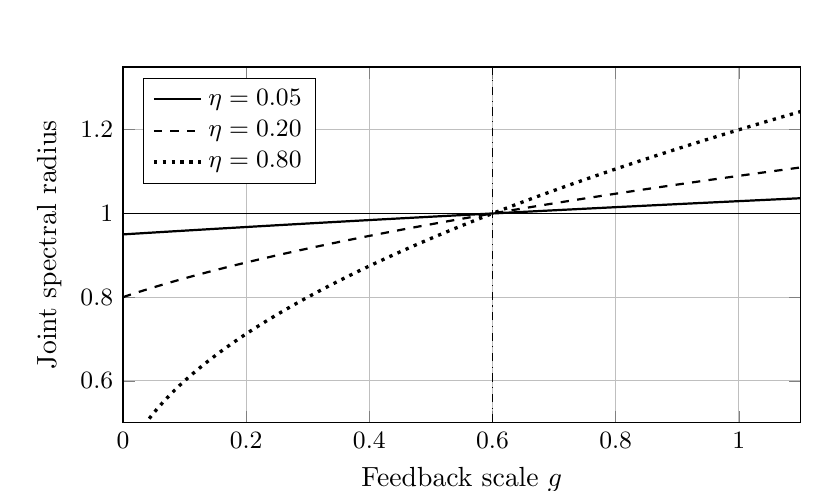
\begin{tikzpicture}
\begin{axis}[width=0.84\textwidth,height=6.1cm,
 xlabel={Feedback scale $g$},ylabel={Joint spectral radius},
 xmin=0,xmax=1.1,ymin=0.5,ymax=1.35,
 legend pos=north west,legend style={font=\small},
 tick label style={font=\small},grid=major]
\addplot[black,thick,domain=0:1.1,samples=120]
 {(0.4+1-0.05+sqrt((0.4-1+0.05)^2+4*x*0.05))/2};
\addlegendentry{$\eta=0.05$}
\addplot[black,dashed,thick,domain=0:1.1,samples=120]
 {(0.4+1-0.2+sqrt((0.4-1+0.2)^2+4*x*0.2))/2};
\addlegendentry{$\eta=0.20$}
\addplot[black,dotted,very thick,domain=0:1.1,samples=120]
 {(0.4+1-0.8+sqrt((0.4-1+0.8)^2+4*x*0.8))/2};
\addlegendentry{$\eta=0.80$}
\addplot[black,thin,forget plot] coordinates {(0,1)(1.1,1)};
\addplot[black,dashdotted,thin,forget plot] coordinates {(0.6,0.5)(0.6,1.35)};
\end{axis}
\end{tikzpicture}
\caption{Analytic illustration for $a=0.4$, $\kappa=1$. The three update rates share the boundary $g=0.6$ but yield different growth or decay rates. No AI models were trained to produce this figure.}
\label{fig:boundary}
\end{figure}

\section{Measurement and causal identification}
\label{sec:measurement}
\subsection{Machine autonomy exposure without arbitrary category scores}
Rather than assign unvalidated values such as $0.1$ to advisory software and $0.7$ to execution software, define a decision event and audit who had executable authority. For event $e$, let $v_e\geq0$ be a predeclared exposure weight and $d_e\in\{0,1\}$ indicate machine execution without a contemporaneous discretionary human approval. For a window $W$,
\begin{equation}
 \MAE_W=\frac{\sum_{e\in W}v_e d_e}{\sum_{e\in W}v_e}.
 \label{eq:mae}
\end{equation}
The denominator must be positive, and weights should represent comparable exposure, not arbitrary numbers of messages. Advisory use, order generation, execution authority, and online learning should be reported separately. Net exposure, gross executed exposure, and assets under management answer different questions and should not be mixed.

If authority is unobserved for some events, report an interval: the lower bound treats unknown events as nonautonomous and the upper bound treats them as autonomous. This makes missingness visible rather than assigning undocumented scores. It does not solve measurement error in $v_e$.

\subsection{Behavioral concentration is not provider concentration}
Provider concentration and common-cloud dependence are operational quantities. Behavioral concentration instead asks whether agents react along similar directions. Let $r_i\in\R^K$ be a nonzero response vector for agent $i$ on an independently designed panel of controlled perturbations, normalized to unit length after reporting its original response magnitude. With $w_i\geq0$ and $\sum_iw_i=1$, define
\begin{equation}
 S=\sum_i w_i r_i r_i^\top,\quad
 \ADC=\lambda_{\max}(S),\quad
 D_{\mathrm{eff}}=\frac{1}{\tr(S^2)}.
 \label{eq:adc}
\end{equation}
Here $\tr(S)=1$, so $\ADC$ is a directional-concentration descriptor. Zero-response agents require a separate reported mass; silently normalizing them is invalid. The perturbation panel, units, weights, and sampling variability all affect the estimate.

There is an important limitation. Two equal-weight agents with responses $r,r$ and two with responses $r,-r$ both yield the same $S$ and $\ADC=1$. Yet their aggregate signed responses are $r$ and zero, respectively. Thus \cref{eq:adc} cannot substitute for the signed aggregate response, price-impact direction, or the product $BC$. Diversity can remove reinforcing feedback, but it can also remove stabilizing behavior. There is no unconditional ``more diversity is safer'' theorem here.

\subsection{An identification impossibility without provenance}
\begin{proposition}[Observational equivalence of decision-maker labels]
\label{prop:identification}
Consider two economies with the same initial market-state distribution, the same market transition kernel conditional on aggregate actions, and the same conditional law of aggregate actions given every observable history. The economies can have different assignments of human and machine decision-maker labels. They nevertheless induce the same law for all observable market histories. No estimator using only those histories can consistently distinguish the two label assignments or identify different autonomy shares attached solely to those assignments.
\end{proposition}
\begin{proof}
The initial observable distributions coincide. If observable histories coincide in distribution through $t$, the assumed conditional action law and common market transition kernel imply the same distribution for the next observation. Induction establishes equality of all finite-dimensional observable distributions. Any statistic of those observations therefore has the same law in both economies; it cannot converge in probability to two distinct label-dependent constants.
\end{proof}
This is an application of ordinary observational equivalence, not a claim that financial attribution is impossible with richer data. Account-level decision provenance, randomly assigned architecture, authorized policy-update experiments, or credible external variation can break the equivalence. Historical prices alone do not reveal whether a self-exciting pattern was produced by humans, fixed algorithms, adaptive agents, or a mixture.

\subsection{Estimating the response system}
The general operator-estimation problem below is broader than the completed scalar experiment. Sections~\ref{sec:observable_protocol}--\ref{sec:observable_results} provide one restricted solution using signed filled probes and prices; they neither reconstruct every private policy state nor identify AI participation from prices alone.

In a simulator with full state access, estimate $J$ by perturbing each normalized coordinate around a specified operating point and measuring the resulting joint next-state response. Use multiple perturbation sizes to test local linearity and independent random streams to quantify agent stochasticity. Finite differences of a mean response estimate a mean-map derivative, not a pathwise derivative of a discrete sampled action.

In observational data, fitting $z_{t+1}=Jz_t+e_{t+1}$ requires sufficient excitation, a defensible state representation, and restrictions controlling confounding and feedback-induced endogeneity. Hidden policy states typically require a state-space or input--output model. A reduced-form estimate may predict outcomes without identifying architecture-specific mechanisms; the paper must report which claim its design supports.

An uncertainty set $\mathcal J$ should reflect estimation uncertainty and relevant model misspecification. There is no distribution-free license to assign a narrow confidence interval to $\rho(J)$ by ignoring dependence, near-defective matrices, hidden states, or selected operating points. A claim of pre-crisis warning additionally requires lead time, false-alarm rates, and a prospectively fixed event definition.

\section{Hidden slow learners: the first companion study}
\label{sec:integrated_hidden}
This section integrates the results of \emph{Hidden Slow Learners}, the first executed companion to the framework \citep{legacy_hidden}. Its purpose is to distinguish a well-defined stability target from the information available to estimate it. The finite-window construction, its limitations, and its adverse controls are retained; they are not treated as newly observed financial facts.

\subsection{Heterogeneous memory and the scalar stability target}
Consider the fixed positive linear specialization
\begin{align}
 x_{t+1}&=a x_t+\sum_{i=1}^n y_{i,t}+\kappa u_t+e_{t+1},\\
 y_{i,t+1}&=(1-\eta_i)y_{i,t}+\eta_i q_i x_t,
 \label{eq:heterogeneous}
\end{align}
where $0\le a<1$, $q_i\ge0$, $0<\eta_i\le1$, and $\kappa>0$. Positivity refers to transition coefficients, not to signs of realized price deviations or positions. Define $Q=\sum_iq_i$ and $G=Q/(1-a)$. Throughout the new experiments, $S=a+Q$ is the unnormalized stability target and $G$ is used only to index generating configurations. Confusing $G$ with $Q$ changes the threshold.

\begin{proposition}[Positive heterogeneous-memory boundary]
\label{prop:heterogeneous_boundary}
The joint transition matrix of \eqref{eq:heterogeneous} is Schur stable exactly when $S=a+Q<1$. Equality gives an eigenvalue at one; $S>1$ gives spectral radius greater than one.
\end{proposition}
\begin{proof}
The matrix is $J=\left[\begin{smallmatrix}a&\mathbf1^\top\\\operatorname{diag}(\eta)q&\operatorname{diag}(1-\eta)\end{smallmatrix}\right]$. The lower diagonal block of $I-J$ is positive. Its Schur complement is $1-a-\sum_iq_i$. The nonsingular M-matrix characterization of a nonnegative transition matrix establishes the stable case. At equality, $(1,q^\top)^\top$ is an eigenvector. Above the boundary, the function
\[
 f(\lambda)=\lambda-a-\sum_i\frac{\eta_iq_i}{\lambda-1+\eta_i}
\]
is negative at one, strictly increasing on $[1,\infty)$, and tends to infinity. It therefore has a root greater than one. This is a specialization of standard positive-system analysis, not a new general stability principle \citep{rantzer2015}.
\end{proof}

With zero initial adaptive states, the loop-open kernel and unit closed-loop response are
\begin{align}
 k_j&=\sum_iq_i\eta_i(1-\eta_i)^j,\quad \sum_{j=0}^{\infty}k_j=Q,\label{eq:integrated_kernel}\\
 h_0&=1,\quad h_1=a,\quad
 h_{t+1}=a h_t+\sum_{j=0}^{t-1}k_jh_{t-1-j}.\label{eq:integrated_h}
\end{align}
The kernel sum exists even when the closed loop is unstable. Summing a diverging closed-loop response and calling it $Q$ would be incorrect.

\subsection{Exact finite-window ambiguity}
\begin{theorem}[Retained exact construction]
\label{thm:retained_pair}
For every positive integer $K$ and $a\in[0,1)$, there are a stable and an unstable model of \eqref{eq:heterogeneous} with the same $a$, the same impact normalization, and the same number of active memory states, whose kernels agree for $j=0,\ldots,K-1$ and whose price responses agree for $t=0,\ldots,K+1$. Rational nodes and $a$ give rational coefficients.
\end{theorem}
\begin{proof}
Choose distinct $0\le r_0<\cdots<r_K<1$ and let
\[
 w_i=\left[\prod_{\ell\ne i}(r_i-r_\ell)\right]^{-1}.
\]
Comparing the leading coefficients in polynomial interpolation gives $\sum_iw_ir_i^j=0$ for $j<K$ and $\sum_iw_ir_i^K=1$. Partial fractions evaluated at one give
\[
 \sum_i\frac{w_i}{1-r_i}=\frac{1}{\prod_i(1-r_i)}>0.
\]
Set $B_+=\sum_i\max(w_i,0)/(1-r_i)$, $B_-=\sum_i\max(-w_i,0)/(1-r_i)$ and $s=2(1-a)/(B_++B_-)$. Alternating signs imply $B_+>B_->0$. Choose $\eta_i=1-r_i$ and $q_i^\pm=s\max(\pm w_i,0)/(1-r_i)$. The totals have midpoint $1-a$ and lie on opposite sides of it. Their kernel difference is $s\sum_iw_ir_i^j$, so the stated terms coincide. Equation~\eqref{eq:integrated_h} propagates this equality to the price responses, with first unmatched difference $h^+_{K+2}-h^-_{K+2}=s$. Delete zero weights and split positive weights among identical-rate copies until each model has $K+1$ active states; splitting changes neither kernel nor stability. Rationality is immediate.
\end{proof}

Equal deterministic observations imply balanced forced-classification error $1/2$ on this pair, even after adding identically distributed observation noise. This is a finite-window, increasing-order construction, not a result that every known low-order market remains unidentifiable indefinitely. Under a fixed valid learning-rate floor below one the construction remains possible, but the stability separation can shrink. A floor is useful for bounds, not a guarantee of finite-sample decisiveness arbitrarily near the boundary.

\begin{table}[htbp]
\centering\small
\caption{Retained readable witness. Four initial price coefficients match exactly.}
\label{tab:retained_witness}
\begin{tabular}{lrr}\toprule
Quantity & Stable member & Unstable member\\\midrule
$a$ & $2/5$ & $2/5$\\
$Q$ & $12/65$ & $66/65$\\
$S=a+Q$ & 0.584615 & 1.415385\\
$\rho(J)$ & 0.757909 & 1.032345\\
$h_0,h_1$ & $1,\ 0.4$ & $1,\ 0.4$\\
$h_2,h_3$ & $0.252308,\ 0.184$ & $0.252308,\ 0.184$\\
$h_4$ & 0.138428 & 0.159198\\\bottomrule
\end{tabular}
\end{table}
Before equal-count splitting, the witness uses rates $(1,1/2,1/20)$ with weights $(0,12/65,0)$ and $(54/1235,0,240/247)$. Displayed decimals are rounded; the equality is rational, not an approximate visual match. A one-rate extrapolation from two exact taps yields
\[
 \widehat Q_{\mathrm{one}}=\frac{k_0^2}{k_0-k_1}\le Q.
\]
Indeed, with $p_i=q_i\eta_i/k_0$, Jensen's inequality for $r\mapsto1/(1-r)$ gives the bound. The inequality is strict for heterogeneous active rates. Thus a low one-rate estimate can be false reassurance, not a stability certificate.

\subsection{What the first measurement experiment actually assumed}
If $\eta_i\ge\underline\eta>0$, $r=1-\underline\eta$, and $T_H=\sum_{j<H}k_j$, positivity gives
\begin{equation}
 T_H\le Q\le\min\left\{\frac{T_H}{1-r^H},\ T_H+\frac{r}{\underline\eta}k_{H-1}\right\}.
 \label{eq:retained_tail}
\end{equation}
These inequalities follow directly by summing each geometric component and bounding its omitted tail. They are not optimal use of the entire moment sequence.

The first companion ran 112 exact paired constructions, 336 common-shock comparisons, and 21,600 noisy measurement datasets across 108 configurations. Its three-way rule made no wrong confident call in that run, with decision coverage of 82.69\% and 66.20\% in the lower- and higher-noise conditions at 256 taps. Those measurements were \emph{loop-open kernel responses with known noise standard error}; they were not ordinary price records. The first paper explicitly warned that deconvolving noisy prices would not preserve that noise model. A falsely specified rate floor could label an unstable model stable. These limitations motivate the next two stages rather than disappearing in the integrated manuscript.

\section{Full-horizon identification audit and fixed-order limits}
\label{sec:integrated_audit}
The second companion, \emph{Hidden Slow Learners Revisited}, audited the first diagnostic using stronger equal-information alternatives \citep{legacy_audit}. Its unfavorable comparison for the original method is retained here. A difficult identification problem does not establish superiority of a particular estimator.

\subsection{A conventional full-information comparison}
All methods received the same noisy normalized kernel vector $\widehat g_j$, known common standard error $v$, and a valid $\underline\eta$, where $g_j=k_j/(1-a)$. Neither generating weights, rates, component count nor class label was supplied. A nonnegative least-squares mixture fit used all observed taps. A second comparator bounded $G$ over positive mixtures consistent with simultaneous confidence intervals, using continuous rate bins to protect off-grid modes. For a feature $f$ and mass $w_l$ in bin $B_l$, its outer inequalities were
\[
 \sum_l \min_{\eta\in B_l} f(\eta)w_l\le U_f,
 \qquad
 \sum_l \max_{\eta\in B_l} f(\eta)w_l\ge L_f.
\]
This belongs to the established set-membership and positive-measure optimization tradition \citep{kosut1992,bertsimas2005}. Stable-model fitting alone would not be an acceptable comparator for detecting instability; stability was not imposed in these fits.

\begin{table}[htbp]
\centering\small
\caption{Retained full-horizon audit at 256 taps. Each noise condition contains 10,800 vectors. These are the earlier kernel measurements, not the new price experiment.}
\label{tab:retained_comparison}
\begin{tabular}{p{.40\textwidth}rrrr}\toprule
 & \multicolumn{2}{c}{Lower noise} & \multicolumn{2}{c}{Higher noise}\\
Method & Decisive (\%) & Wrong & Decisive (\%) & Wrong\\\midrule
Original summary bound & 82.69 & 0 & 66.20 & 0\\
Full-horizon positive point fit & 100.00 & 24 & 100.00 & 306\\
Full-moment positive bounds & 88.04 & 0 & 76.65 & 4\\\bottomrule
\end{tabular}
\end{table}

The bounds resolved 578 and 1,128 additional vectors respectively, but did not dominate on every realization. Some earlier decisions became model conflicts, and four high-noise decisions were wrong. All four occurred outside the simultaneous confidence event. Across the 82,364 rows on that event, the reported interval contained the true gain and made no wrong confident call. The full audit comprised 86,400 rows over four horizons. Its strongest interpretation is a measurement requirement and benchmark, not an improved original summary diagnostic.

\subsection{A fixed-order lower bound in the earlier observation law}
For two common-rate models with rates $(1/2,\eta)$ and normalized weights $(0.7,0.2)$ and $(0.7,0.4)$, the gains are $0.9$ and $1.1$. With $\Delta=0.2$, their kernel means differ by $\Delta\eta(1-\eta)^j$. Under \emph{independent kernel noise} of variance $v^2$, their squared Mahalanobis distance is
\begin{equation}
 d_{H,\mathrm{kernel}}^2=
 \frac{\Delta^2\eta\{1-(1-\eta)^{2H}\}}{v^2(2-\eta)}.
 \label{eq:kernel_distance_retained}
\end{equation}
The equal-prior optimal forced error is $\Phi(-d/2)$, obtained by projecting onto the standardized mean difference. If a rule may abstain, its balanced decision coverage $c$ and unconditional wrong-label probability $e$ obey
\begin{equation}
 c\le \min\{1,\,2e+2\Phi(d/2)-1\}.
 \label{eq:retained_coverage_limit}
\end{equation}
For disjoint stable and unstable decision regions, subtract twice the error from coverage and bound the difference of probabilities by total variation. The Gaussian total variation is $2\Phi(d/2)-1$. This is a direct specialization of classical two-point testing, not a new general lower-bound method; identification sample-complexity precedents must also be acknowledged \citep{jedra2019}.

At $\eta=10^{-5}$, $H=256$, $v=0.02/\sqrt{128}$, the oracle error is 49.6394\%. An unconditional error target of 5\% permits at most 10.7212\% coverage on that pair. Because this particular kernel experiment adds equally noisy late taps, its information can saturate. \textbf{These numbers and the saturation conclusion must not be transferred unchanged to a different price-measurement protocol.} The price experiment below has a different observation law and a separately calculated lower bound.

\section{An observable intervention protocol without hidden-state access}
\label{sec:observable_protocol}
The new research step replaces assumed kernel observations with recorded probe fills and quoted prices. It does not identify the full latent Jacobian or the fraction of trades performed by AI. It estimates an input--output response and asks what that response supports about $S$ under the declared positive-memory class. This change is compatible with established data informativity: a property can sometimes be determined without uniquely recovering every parameter \citep{vanwaarde2020}.

\subsection{Information available to the estimator}
In each of $R$ independent episodes, assign one signed pulse $u_r\in\{-\delta,+\delta\}$, balanced across signs and randomized independently of the initial latent states and subsequent disturbances. Record the \emph{filled quantity}, not merely the intended order, and the subsequent quote changes $Y_{r,j}=P_{r,j+1}-P_{r,0}$, $j=0,\ldots,M-1$. Within a linear time-invariant episode,
\begin{equation}
 Y_{r,j}=m_j+u_r\beta_j+\varepsilon_{r,j},
 \qquad \beta_j=\kappa h_j.
 \label{eq:public_measurement}
\end{equation}
The arbitrary common intercept path $m_j$ accommodates the mean no-probe trajectory. The estimator receives only $(u_r,Y_{r,\cdot})$ and a valid externally declared $\underline\eta$. It receives neither private states, private aggregate pressures, exact rates, weights, $a$, $\kappa$, nor the disturbance variance. Initial adaptive states need not be zero or observable: in the experiment they are independent Gaussian draws, hidden from the estimator.

For the exact confidence result, episodes have independent identically distributed Gaussian residual vectors $\varepsilon_r\sim N(0,\Sigma)$, independent of assignment, where $\Sigma$ is unknown and may have arbitrary temporal covariance. This is a finite-window condition; it does not require stationary prices or closed-loop stability. Gaussian initial states, additive flow disturbances and quote errors in the fixed linear simulator imply it. It is not guaranteed by a successful regression on a real market.

\subsection{Recovering the response and its uncertainty}
Let $v_r=u_r-\bar u$ and $D=\sum_r v_r^2>0$. Ordinary regression with an intercept gives
\begin{align}
 \widehat\beta_j&=D^{-1}\sum_r v_rY_{r,j},\qquad
 \widehat m_j=\bar Y_j-\bar u\widehat\beta_j,\\
 \widehat\Sigma&=\frac1{R-2}\sum_r
 (Y_r-\widehat m-u_r\widehat\beta)
 (Y_r-\widehat m-u_r\widehat\beta)^\top,\\
 \widehat{\operatorname{Cov}}(\widehat\beta)&=\widehat\Sigma/D.
 \label{eq:observed_covariance}
\end{align}
The covariance is estimated from public price residuals; no oracle covariance is inserted. For balanced pulses, $D=R\delta^2$. Repeating episodes and increasing pulse size change precision, but larger pulses can invalidate linearity and create additional economic exposure.

\begin{theorem}[Finite-family response uncertainty]
\label{thm:observable_ci}
Under \eqref{eq:public_measurement} and the stated independent Gaussian episode contract, let
\[
 z=t_{R-2}^{-1}\!\left(1-\frac{\alpha}{2M}\right),\qquad
 L_j=\widehat\beta_j-z\sqrt{\widehat\Sigma_{jj}/D},\quad
 U_j=\widehat\beta_j+z\sqrt{\widehat\Sigma_{jj}/D}.
\]
Then $\mathbb P(\beta_j\in[L_j,U_j]\ \text{for all }j<M\mid u)\ge1-\alpha$. No temporal independence between price observations or between estimated response coefficients is required.
\end{theorem}
\begin{proof}
Conditional on the nonconstant design, each response coordinate is a Gaussian regression with two fitted coefficients. Its standardized slope error has a Student-$t$ distribution with $R-2$ degrees of freedom; the residual variance is independent of that coordinate's slope estimate. Each two-sided interval fails with probability $\alpha/M$. A union bound over the $M$ coordinates yields the result even though these statistics are dependent. In a noiseless coordinate the interval degenerates to its exact coefficient. This is an application of ordinary Gaussian regression inference, not a claim to a new distribution-free method. Exact finite-sample methods under other assumptions already exist, including sign-perturbed sums \citep{csaji2015}.
\end{proof}

The event covers all predeclared horizons that use these same coefficients. It is not anytime-valid for an unlimited search over new windows, budgets or operating points. A 95\% guarantee applies separately to a declared measurement panel, not simultaneously to the entire collection of thousands of simulation panels. It is also an unconditional wrong-label bound, not a 5\% conditional error guarantee among the few cases that receive labels.

\subsection{Exact deconvolution is possible; independent noise is not preserved}
With exact response coefficients and $\beta_0>0$, the unknown impact and direct persistence are recoverable:
\begin{equation}
 \kappa=\beta_0,\quad h_j=\beta_j/\beta_0,\quad a=h_1,\quad
 k_n=h_{n+2}-a h_{n+1}-\sum_{j=0}^{n-1}k_jh_{n-j}.
 \label{eq:observable_deconvolution}
\end{equation}
Thus finite loop-open responses can be obtained without observing the adaptive states. The exact claim is algebraic; noisy point estimates require uncertainty propagation. For example,
\[
 k_0=\frac{\beta_2}{\beta_0}-\left(\frac{\beta_1}{\beta_0}\right)^2,
\]
whose gradient with respect to $(\beta_0,\beta_1,\beta_2)$ is
\[
 \left(-\frac{\beta_2}{\beta_0^2}+\frac{2\beta_1^2}{\beta_0^3},
 -\frac{2\beta_1}{\beta_0^2},\frac1{\beta_0}\right).
\]
Even a first-order variance approximation uses the \emph{full} response covariance. Recursive products, division by a weak initial response and dependence across times can amplify uncertainty. Reusing the previous iid-kernel Gaussian endpoints on these estimates would be unjustified. The new pipeline therefore avoids requiring a precise point estimate of every $k_n$.

\section{Positive recurrence bounds directly from uncertain prices}
\label{sec:observable_bounds}
This section constructs an outer feasible set directly from the response intervals, following conventional set-membership logic. The relevant methodological increment in this artifact is the explicit link from randomized price measurements to that set, including unknown persistence and impact. Neither broad novelty nor optimality over all input--output estimators is asserted.

\subsection{A response-only convex outer relaxation}
The response satisfies
\begin{equation}
 \beta_{t+1}=a\beta_t+\int_{\underline\eta}^{1}
 \left[\sum_{j=0}^{t-1}\eta(1-\eta)^j\beta_{t-1-j}\right]d\mu(\eta),
 \quad \mu=\sum_iq_i\delta_{\eta_i},
 \label{eq:public_recurrence}
\end{equation}
with an empty sum at $t=0$. This equation is homogeneous in the price-impact scale; there is no need to divide a noisy record by an assumed known $\kappa$.

Intersect response lower bounds with zero, since the theoretical impulse response is nonnegative. An upper bound below zero is a model conflict. If $L_0\le0$, the present implementation remains inconclusive rather than normalizing by a poorly supported impact. Partition $[\underline\eta,1]$ into bins $B_l$ and let $w_l=\mu(B_l)\ge0$. For $\psi_j(\eta)=\eta(1-\eta)^j$ define exact endpoint/peak bounds
\[
 \psi_{jl}^-=\min_{\eta\in B_l}\psi_j(\eta),\qquad
 \psi_{jl}^+=\max_{\eta\in B_l}\psi_j(\eta).
\]
The minimum is at an endpoint; the maximum is at the projection of $1/(j+1)$ onto the bin. Set
\begin{equation}
 C_{tl}^-=\sum_{j=0}^{t-1}\psi_{jl}^-L_{t-1-j},\qquad
 C_{tl}^+=\sum_{j=0}^{t-1}\psi_{jl}^+U_{t-1-j}.
\end{equation}
Every compatible true model then satisfies the \emph{linear} inequalities
\begin{align}
 aL_t+\sum_l C_{tl}^-w_l&\le U_{t+1},\\
 aU_t+\sum_l C_{tl}^+w_l&\ge L_{t+1},\qquad 0\le a\le1,
 \quad w_l\ge0.
 \label{eq:price_outer}
\end{align}
Minimize and maximize $a+\sum_lw_l$ over this set to obtain $[S_-,S_+]$. Different terms may attain their bin extrema at different rates and different response endpoints; the relaxation is conservative, not an exact description of all realizations. Refining bins does not by itself remove the looseness of rectangular response uncertainty.

\begin{theorem}[Observable-data stability interval]
\label{thm:observable_stability}
Under the model, a valid rate floor, and the response event in Theorem~\ref{thm:observable_ci}, the true $S$ belongs to $[S_-,S_+]$ in exact arithmetic at every declared horizon. Declaring stable if $S_+<1$, unstable if $S_->1$, and otherwise inconclusive therefore has probability at most $\alpha$ of any wrong confident label within the declared family.
\end{theorem}
\begin{proof}
On the response event, all true $\beta_t$ lie in the clipped nonnegative intervals. Positivity of $a$, the kernel and bin masses makes each lower convolution no greater than its true value and each upper convolution no smaller. Thus the true $(a,w)$ satisfies \eqref{eq:price_outer}. Its objective is exactly $a+\mu([\underline\eta,1])=S$, so the LP extremal values enclose it. Proposition~\ref{prop:heterogeneous_boundary} gives the label implication; the probability statement follows from the simultaneous event. Unknown hidden states affect the observational residual distribution, not the feasibility proof, provided they satisfy the independent episode contract.
\end{proof}

A useful numerical anchor follows from $\beta_2\ge\underline\eta\,\beta_0Q$:
\begin{equation}
 S\le 1+\frac{U_2}{\underline\eta L_0},\qquad L_0>0.
 \label{eq:observable_cap}
\end{equation}
The implementation includes this redundant true-model bound, outward feature padding, dual residual repair, primal/dual checks and a $10^{-7}$ classification margin. Linear-programming bounds are guarded numerically, not formally verified with interval arithmetic. Solver failure and infeasibility are not converted into a favorable label.

\subsection{Equal observable-information comparators}
The first comparator propagates the same response rectangle through \eqref{eq:observable_deconvolution}, intersects each kernel interval with positivity, and applies \eqref{eq:retained_tail}. It is conservative but repeatedly reuses uncertain quantities, so interval widths can grow sharply. The second is a conventional positive recurrence least-squares fit using all response coefficients and a 33-node rate grid. It fits $a\in[0,1]$ and nonnegative weights without imposing $a+Q<1$.

The point fit uses measured response coefficients on both sides of a regression, creating an errors-in-variables problem. It is not a calibrated certificate, not a strongest possible nonlinear output-error estimator, and not a replacement for the full-horizon kernel audit. The comparison asks whether this explicit measurement protocol can yield valid intervals and what it costs in undecided cases. It does not establish superiority to every conventional identification method. Existing positivity- and gain-informed identification is a necessary comparison literature \citep{khosravi2025,khosravi2022}.

\section{An account-consistent market environment}
\label{sec:economic_measurement}
To attach the response to economic transactions, the new experiment implements a stylized dealer market rather than feeding the estimator noisy kernel coefficients. It is an excess-demand price-adjustment model with explicit trades and ledgers, not a calibrated exchange or a limit-order book.

\subsection{Orders, price formation and adaptive demand}
Let $P_t=p^*+x_t$, with the constant reference value $p^*=100$ dollars. Chartist $i$ holds a private smoothed displacement $m_{i,t}$, with demand $v_{i,t}=\chi_i m_{i,t}$. A fundamentalist submits $v_{F,t}=-\varphi x_t$, a noise trader submits $v_{N,t}$, and the experiment's trader submits $u_t$. The dealer absorbs their net quantity $V_t$. Prices and memories update as
\begin{align}
 V_t&=\sum_i v_{i,t}+v_{F,t}+v_{N,t}+u_t,\qquad
 P_{t+1}=P_t+\kappa V_t,\\
 m_{i,t+1}&=(1-\eta_i)m_{i,t}+\eta_i x_t.
 \label{eq:economic_orders}
\end{align}
Writing $a=1-\kappa\varphi$, $q_i=\kappa\chi_i$ and $y_{i,t}=\kappa\chi_i m_{i,t}$ gives \eqref{eq:heterogeneous} exactly. Updates use $x_t$, not the newly moved $x_{t+1}$; changing timing changes the response recurrence. Agents have adaptive memory, not trained neural policies or demonstrated utility-optimal behavior.

Empirical order-book research motivates considering a local relation between net pressure, price changes and depth, but does not validate this specific aggregate-demand model or its chosen parameters \citep{cont2014}. In particular, actual order-flow imbalance includes quote and cancellation events; the simple signed trade volume $V_t$ here is not claimed to equal that empirical measure.

\subsection{Double-entry accounting and economic scope}
Trades execute at the within-step midpoint $P_t^{\rm ex}=(P_t+P_{t+1})/2$, with half-spread $c=0.005$ dollars transferred to the dealer. Each nondealer actor with quantity $v$ has changes
\[
 \Delta N=v,\qquad \Delta C=-vP_t^{\rm ex}-c|v|.
\]
The dealer has the opposite aggregate inventory and cash changes. Thus total shares and cash transfers sum to zero after every step; marking all inventories to one common quote also preserves aggregate marked wealth when net initial shares are zero. The cash variables are ledger changes, not evidence that all actors satisfy capital requirements. Unconstrained credit and short positions, fixed depth, no defaults and no endogenous balance-sheet limits make the primary model a local mechanism test rather than a complete financial economy.

The primary price impact is $0.02$ dollars per share and $a=0.4$, implying $\varphi=30$ shares per dollar. Chartist elasticities are set from the declared $q_i$. Background net-flow noise has standard deviation 0.10 shares; quote observation error has standard deviation 0.002 dollars; each initial private memory has standard deviation 0.01 dollars. The estimator is not told these scales. Time is an abstract model step, not a claimed number of market seconds. No live-market orders, customer records or external financial data are used.

\subsection{Experimental design and information firewall}
The frozen primary panel uses rates $(0.5,\eta_s)$ with $\eta_s\in\{0.002,0.02,0.10\}$ and $G\in\{0.70,0.95,1.05,1.30\}$. Sixty percent of normalized feedback is fast and forty percent slow. The imposed class floor is $\underline\eta=\eta_s$; this is public design-side information, not an estimated individual hidden rate. The equality at the floor is a benchmark boundary choice, and off-grid support is separately tested.

For each of 12 configurations, 128 or 1,024 independent episodes use pulses of one or four shares. Forty independent panels per configuration/design give 1,920 panels. Each episode records 66 quote changes. Inference at largest lags 8, 24 and 64 gives 5,760 horizon rows. There are $H+1$ response coefficients through lag $H$; the last collected coefficient, lag 65, is unused in these fits but included in the simultaneous confidence family, conservatively. There are 1,105,920 episodes and 72,990,720 quoted-price observations, not that many independent financial markets.

Only a public object with keys \texttt{probes} and \texttt{prices} crosses into estimation. Analytical responses, latent trajectories, true gains and configuration labels are used by the evaluation layer only. Known noise standard deviations and exact direct persistence are not estimator arguments. Full public response estimates, endpoints and standard errors are saved for every panel, together with generation seeds and raw-record hashes. Four public episode examples and their response covariances are included. All other raw episodes can be regenerated; they are not represented as external market records.

\section{Executed observable-data findings}
\label{sec:observable_results}
\subsection{Response recovery and confidence calibration}
The simultaneous response intervals covered all 66 true coefficients in 1,895 of 1,920 panels, or 98.70\%, versus a nominal lower coverage of 95\%. Estimated neighboring response errors were strongly correlated: the mean absolute adjacent correlation was 0.8497. This supports the decision not to reuse an iid-kernel error model. These are measurements from the declared synthetic experiment, not estimates of correlations in a real exchange.

On all 5,685 horizon rows whose panel satisfied the response event, the output-only recurrence interval contained the true $S$. It made no wrong confident call anywhere in the 5,760 primary rows, including the 75 rows from the 25 panels outside that event. The observed absence of errors is not proof of a zero-error procedure.

\begin{table}[htbp]
\centering\small
\caption{New price-only experiment at largest fitted lag 64. Each row contains 480 panels. Parentheses show wrong labels; point fitting always gives a label but has no confidence guarantee.}
\label{tab:observable_primary}
\begin{tabular}{rr rrr}\toprule
Episodes & Pulse (shares) & Recurrence bound & Interval deconvolution & Point fit\\\midrule
128 & 1 & 0/480 (0) & 0/480 (0) & 480/480 (101)\\
128 & 4 & 28/480 (0) & 0/480 (0) & 480/480 (56)\\
1,024 & 1 & 0/480 (0) & 0/480 (0) & 480/480 (49)\\
1,024 & 4 & 80/480 (0) & 0/480 (0) & 480/480 (37)\\\bottomrule
\end{tabular}
\end{table}

The strongest primary design therefore resolves 16.67\%, leaving 83.33\% inconclusive. All 80 decisions in that design occur at the fastest allowed slow rate, $\eta_s=0.10$, and the large-margin gains $G=0.70$ and $1.30$, with 40 correct decisions each. Neither near-boundary gain nor either slower class is resolved by that design. Across all three nested horizons, the recurrence method makes 256 decisions (176 stable and 80 unstable) and leaves 5,504 rows inconclusive. Nested horizon decisions are not independent replications.

The naive interval-deconvolution comparator remains inconclusive throughout the primary panel. This is evidence of looseness in that particular interval propagation, not a theorem that all deconvolution methods fail. The point estimator makes 1,191 wrong labels across the 5,760 rows. Its apparent 100\% decisiveness is therefore not a substitute for a supported stability statement. Nor is this weak point comparator a basis for claiming superiority over the strongest output-error or covariance-aware conventional methods.

\subsection{Replication budget and the cost of a useful answer}
After inspecting primary results, a separately labeled exploratory extension uses 8,192 and 32,768 episodes, four-share pulses and largest lag 64. Five panels per configuration/budget give 60 panels at each budget. There are 15/60 (25.00\%) and 25/60 (41.67\%) definite answers, with no wrong labels. At 32,768 episodes all 20 fastest-class panels are resolved, five moderate-rate stable large-margin panels are resolved, and all 20 slowest-class panels remain inconclusive. The extension contributes 2,457,600 simulated episodes but is not pooled with the frozen primary analysis.

These results expose an observation-budget problem, but low decisiveness also reflects conservative bin/rectangle relaxation and discarded covariance geometry. They do not prove that the remaining cases are information-theoretically impossible at these budgets. A full-covariance, positivity-constrained output-error set is an important stronger comparison before attributing all nondecisions to lack of information.

\subsection{Assumption failures are not repaired by good price confidence}
\begin{table}[htbp]
\centering\small
\caption{Twenty panels per control, each with 4,096 episodes and four-share pulses. Controls are not part of the primary calibration claim.}
\label{tab:observable_failures}
\begin{tabularx}{\textwidth}{p{.27\textwidth}YY}\toprule
Condition & Observed result & Interpretation\\\midrule
Valid reference & 20 stable labels; all response bands cover & Consistent with the declared class\\
False rate floor & 20 stable labels for an unstable linear system; all response bands cover & Accurate measured responses do not validate hidden-tail assumptions\\
Confounded assignment & 20 model conflicts; zero response bands cover the causal response & Randomization is part of identification, not decoration\\
Saturating price impact & 20 stable labels; zero bands cover the origin's linear response & A plausible label does not establish linearity or global safety\\\bottomrule
\end{tabularx}
\end{table}

In the false-floor control, actual rates are $(0.5,10^{-5})$ but inference is incorrectly told $\underline\eta=0.10$. Weights $(0.42,0.24)$ give $S=1.06$. All price-response confidence events hold, yet the true measure is excluded from the allowed support and all 20 outputs are falsely stable. No output-only claim here certifies the rate floor itself.

The confounded control assigns signs using future background flow, deliberately breaking independence. The nonlinear control replaces $\kappa V$ by $\kappa c_0\tanh(V/c_0)$ with $c_0=1$ share. Its Jacobian at the origin retains the linear reference, but finite pulses do not. In an exact noise-free scaling check, initial price response per share is 0.0195935, 0.0152319 and 0.00499665 for pulses of 0.25, 1 and 4 shares. A larger pulse improves linear-model signal-to-noise only while linearity remains valid. Passing feasibility is not a model-validation test; failing amplitude invariance can flag a problem but cannot certify the remaining assumptions.

\subsection{A new lower bound for the actual price-observation family}
\label{subsec:price_limit}
To separate observation limits from solver conservatism, consider a restricted subexperiment with zero initial states, no flow noise and independent quote noise $N(0,\sigma^2)$. This subexperiment is not the full noisy-dealer panel. For the two models with $a=0.4$, rates $(0.5,\eta)$ and $q^{(0)}=0.6(0.7,0.2)$, $q^{(1)}=0.6(0.7,0.4)$, define their observable price responses $\beta^{(0)},\beta^{(1)}$ as in \eqref{eq:public_measurement}.

\begin{theorem}[Fixed-budget price-response ambiguity]
\label{thm:price_limit}
With $R$ balanced pulses of magnitude $\delta$, observed through lag $H$, the exact Gaussian distance is
\begin{equation}
 d_{H,\mathrm{price}}^2=\frac{R\delta^2}{\sigma^2}
 \sum_{j=0}^{H}(\beta_j^{(1)}-\beta_j^{(0)})^2.
 \label{eq:price_distance}
\end{equation}
The optimal balanced forced-classification error is $\Phi(-d_{H,\mathrm{price}}/2)$, and the abstention bound \eqref{eq:retained_coverage_limit} holds using this new distance. For fixed $H,R,\delta,\sigma>0$, the distance tends to zero as $\eta\downarrow0$, although the two gains remain $G_0=0.9$ and $G_1=1.1$ and both models have two memory states.
\end{theorem}
\begin{proof}
Conditional on the known assignments, the stacked observation covariance is $\sigma^2I$ and each episode's mean difference is $u_r(\beta^{(1)}-\beta^{(0)})$. Summing squared standardized differences gives \eqref{eq:price_distance}. Projection onto that direction gives the same scalar Gaussian likelihood-ratio calculation as before.

For the limit, let $J_0,J_1$ be the pressure-coordinate matrices in Proposition~\ref{prop:heterogeneous_boundary}. Their difference has a single entry $\eta\Delta q$, where $\Delta q=0.12$. A common induced norm bound $\|J_i\|\le M$ can be chosen independently of $\eta\in(0,1]$. The telescoping identity for powers gives
\[
 \|J_1^j-J_0^j\|\le jM^{j-1}\eta\Delta q.
\]
Since $\beta_j^{(i)}=\kappa e_1^\top J_i^je_1$, every finite coefficient difference tends to zero and so does the finite sum in \eqref{eq:price_distance}. The gains do not depend on $\eta$. This proves the restricted finite-budget impossibility, not a claim about all possible excitation policies.
\end{proof}

For $R=1,024$, $\delta=4$, $\sigma=0.002$, $H=64$, and $\kappa=0.02$, the exact oracle errors are 49.94\%, 49.42\%, 44.27\%, and 7.45\% at rates $10^{-7}$, $10^{-6}$, $10^{-5}$, and $10^{-4}$. At $\eta=10^{-5}$ an unconditional 5\% wrong-label target permits at most 21.46\% balanced decision coverage on this pair. These are newly computed \emph{price-law} examples, not the 49.64\% kernel-law number in the previous audit. The limit lets the allowable slowest rate approach zero; it does not hold that rate above one fixed positive floor while simultaneously sending it to zero. Each numerical pair must be assigned a class floor no greater than its actual slow rate. A 100,000-draw likelihood-score Monte Carlo check accompanies the exact calculation. Neither this limit nor the primary low decisiveness establishes a universal crisis-prediction impossibility.

\subsection{Accounting, numerical checks and reproduction}
Across all primary simulated steps, maximum absolute conservation errors were $3.37\times10^{-11}$ dollars in cash transfers, $3.52\times10^{-13}$ shares and $4.61\times10^{-11}$ dollars in aggregate marked wealth. The largest price displacement was about 1.010 dollars from the artificial 100-dollar reference. These are accounting and implementation checks, not claims of economic realism.

Twenty-two new tests pass, including off-grid feasible-mixture checks, unknown-parameter interface tests, exact response recovery, amplitude scaling and accounting. The previous releases' 29 and 23 tests were rerun and passed; the original 625 scalar and 250 network algebra checks were also rerun. A separately assembled group-means regression agrees to $1.95\times10^{-16}$ on 48 regenerated panels. Alternative interior-point optimization agrees with the main dual-simplex bounds to $1.30\times10^{-12}$ across 144 comparisons. Maximum primary primal residual was $2.23\times10^{-10}$; the guarded dual residual was zero to the reported precision. These are internal cross-checks, not independent outside review.

A second full run in a clean output directory regenerated all primary panels, response summaries and comparison rows. Both panel and comparison CSV files match byte for byte; all nine repeated NPZ datasets match array for array. Runtime is recorded separately and is not expected to match. The supplemental archive contains the versioned protocols, source, tests, all result rows, every public response summary, seed manifests, four complete public example datasets and source-paper provenance. The new study uses NumPy 2.3.5 and SciPy 1.17.0; solver options are recorded rather than relying on changing library defaults \citep{scipy_highs}.


\section{Intervention under uncertainty and liquidity feedback}
\label{sec:intervention}
A proposed intervention can reduce order size, slow an update, retain a previously approved policy, route a decision to review, or abstain from a specific action. These are not interchangeable. In particular, freezing learning need not cancel outstanding orders, and abstaining from new positions need not remove existing inventory risk.

\begin{proposition}[Common-norm robustness; standard sufficient condition]
\label{prop:robust}
Let $P\succ0$, $\norm{z}_P=(z^\top Pz)^{1/2}$, and let $\norm{J}_P$ be the associated induced norm. Suppose all admissible transition matrices satisfy $\norm{J}_P\leq\gamma<1$. For any sequence of those matrices and additive disturbances with $\norm{b_t}_P\leq\bar b$, the system $z_{t+1}=J_tz_t+b_t$ satisfies
\begin{equation}
 \norm{z_T}_P\leq\gamma^T\norm{z_0}_P+
 \bar b\frac{1-\gamma^T}{1-\gamma}.
 \label{eq:robustbound}
\end{equation}
A sufficient estimation-aware test is $\norm{\widehat J}_P+\epsilon\leq\gamma$ when $\norm{J-\widehat J}_P\leq\epsilon$ holds for every admissible $J$.
\end{proposition}
\begin{proof}
Submultiplicativity and the triangle inequality give $\norm{z_{t+1}}_P\leq\gamma\norm{z_t}_P+\bar b$. Iteration yields the geometric bound. The final sufficient test follows from $\norm{J}_P\leq\norm{\widehat J}_P+\norm{J-\widehat J}_P$.
\end{proof}
The common $P$ is essential: separate certificates with incompatible metrics do not certify arbitrary switching. A standard matrix formulation is $J^\top PJ\preceq\gamma^2P$ for every admissible matrix \citep{boyd1994}. In a nonlinear setting, analogous derivative bounds must hold throughout an invariant neighborhood; a certificate at one point is insufficient. A probabilistic estimation set yields only a guarantee conditional on its coverage event and assumptions.

\subsection{Why abstention is not automatically stabilizing}
Consider the scalar positive-feedback model with $a=0.4$, $\eta=0.2$, $\kappa=1$, and baseline $g_0=0.45$. Suppose an intervention retains a fraction $u$ of demand sensitivity but depth falls to a fraction $q(u)$ of baseline. The effective scale becomes
\begin{equation}
 g(u)=g_0\frac{u}{q(u)}.
 \label{eq:gatedepth}
\end{equation}
At $u=0.5$ and unchanged depth, $g=0.225$ and the model is more strongly stable. At $u=0.5$ and $q(u)=0.25$, $g=0.9$ and the model is unstable. These are constructed scenarios, not estimated liquidity elasticities. They show why evaluating abstention only through reduced individual trading ignores an essential equilibrium response.

Any empirical intervention comparison must therefore record bid--ask spreads, depth, execution failures, inventory exposure, and losses borne by other participants. An intervention that reduces one agent's losses by transferring risk or withdrawing market-making capacity is not automatically a system improvement. Operational deployment is outside this manuscript's scope.

\section{Executed numerical checks}
\label{sec:checks}
\subsection{Purpose and reproducibility}
The computations reported here test agreement between formulas and direct matrix calculations. They neither fit the model to a financial dataset nor train financial agents. \Cref{app:code} contains the exact self-contained Python/NumPy program used for the reported matrix checks. The run used NumPy 2.3.5, double-precision arrays, and seed 20260918 for the network samples. Last-digit differences across numerical libraries are immaterial to the stated tolerances.

\begin{table}[htbp]
\centering\small
\caption{Computed scalar-model examples. All rows use $a=0.4$ and $\kappa=1$. Parameters are illustrative and uncalibrated.}
\label{tab:scalar}
\begin{tabularx}{\textwidth}{Yrrrr}
\toprule
Case & $g$ & $\eta$ & $\rho(J_s)$ & $g\kappa/(1-a)$\\
\midrule
Stable feedback & 0.300 & 0.20 & 0.916228 & 0.500\\
Boundary & 0.600 & 0.20 & 1.000000 & 1.000\\
Unstable feedback & 0.900 & 0.20 & 1.069042 & 1.500\\
Same unstable gain, slower learning & 0.900 & 0.05 & 1.022311 & 1.500\\
Same unstable gain, faster learning & 0.900 & 0.80 & 1.154400 & 1.500\\
Baseline before action gate & 0.450 & 0.20 & 0.960555 & 0.750\\
Gate with depth unchanged & 0.225 & 0.20 & 0.891548 & 0.375\\
Gate with depth at one quarter & 0.900 & 0.20 & 1.069042 & 1.500\\
\bottomrule
\end{tabularx}
\end{table}

\subsection{Verification results}
The scalar Cartesian grid comprises five values each of $a$, $\eta$, $g$, and $\kappa$, giving $5^4=625$ cases away from the boundary. All direct eigenvalue classifications agree with $g\kappa<1-a$. The largest absolute difference between the formula and direct eigenvalue calculations is approximately $2.22\times10^{-16}$.

The network check uses 250 independently generated nonnegative pairs with $d=3$ market coordinates and $n=4$ adaptive states, along with randomized admissible scalar parameters. All classifications agree with \cref{eq:boundary}; the largest formula discrepancy is approximately $2.89\times10^{-15}$. These are numerical consistency tests, not 250 independent market experiments and not evidence of generalization to large language models.

The program also verifies the switching example, the transient-amplification example, and the signed-response concentration counterexample. The switching product has spectral radius $4.486068$, corresponding to an asymptotic per-step factor of approximately $2.118034$ under periodic alternation. The stable nonnormal example reaches the previously reported gain $8.212429$. Both identical and opposite response panels have $\ADC=1$, despite different aggregate signed responses.

The mathematical proofs, not the finite grid, justify the universal statements within the specified model. The computations provide an implementation check and reproducible illustrations. No confidence interval or significance claim is attached to an exact algebra check.

\section{Next-stage validation: matched policies, observation limits and operational risk}
\label{sec:next_stage}
This section integrates the separately packaged next-stage validation without pooling its denominators with the earlier observable-price study. It is a scoped evidence layer: the environment, policy family, observation law, intervention target and public-data corpus each have their own counting unit and claim boundary.

\subsection{Matched synthetic policies and training result}
The next-stage environment is an independently specified CPU-only market with explicit price, cash, inventory, spread, depth, impact, partial fills, fees, margin, drawdown and halt logic. The public observation vector contains return, normalized inventory, equity change, spread, depth, margin ratio and normalized time; future shocks and latent states are not exposed. The fixed controller submits no order, the adaptive non-neural controller is a declared linear rule, and the trained controller is a seven-input, eight-hidden-unit tanh policy. Its weights are optimized by deterministic population search on development tapes and frozen for paired held-out evaluation. Capital, information, execution, fees, latency, tapes and evaluation episodes are matched across policies.

The primary estimand is paired neural-minus-adaptive gain in account units. A 0.5-unit mean improvement on a 100-unit account was declared the minimum meaningful effect before the confirmation run. The three seed-level results are:

\begin{table}[htbp]
\centering\small
\caption{Matched-policy confirmation results. Values are mean account gains; intervals are paired bootstrap 95\% intervals for neural minus adaptive gain.}
\label{tab:next_agent}
\begin{tabular}{lrrrr}
\toprule
Training seed & No trade & Adaptive & Neural & Neural--adaptive (95\% interval)\\
\midrule
601 & 0.000 & -0.093 & -0.183 & -0.090 $[-0.980,0.804]$\\
602 & 0.000 & -0.093 & -0.116 & -0.023 $[-0.357,0.314]$\\
603 & 0.000 & -0.093 & -0.045 & 0.048 $[-0.160,0.265]$\\
\bottomrule
\end{tabular}
\end{table}

The macro-average neural-minus-adaptive gain is $-0.022$ and no seed clears the predeclared threshold. This supports a small synthetic null against the matched adaptive controller, not a conclusion that AI systems cannot have an effect. The policy family is narrow, the training is not reinforcement learning, and no empirical-log causal comparison is established.

\subsection{Noisy and dependent observation benchmark}
The observation benchmark generates a declared latent episode process, adds response and regressor noise, optionally introduces within-episode autoregressive dependence, and masks observations. The estimator includes an intercept and resamples complete episodes rather than treating trace rows as independent. Coverage is simulation-calibrated for this law, not an exact theorem or a market estimate.

\begin{table}[htbp]
\centering\small
\caption{Observation diagnostics. The independent unit is an episode; coverage, wrong-confidence and unresolved fractions are separate quantities.}
\label{tab:next_observation}
\begin{tabular}{lrrrr}
\toprule
Condition & Coverage & Decisive & Wrong confident & Unresolved\\
\midrule
Exact independent & 1.000 & 1.000 & 0.000 & 0.000\\
Noisy independent & 0.835 & 1.000 & 0.000 & 0.000\\
Noisy dependent & 0.795 & 1.000 & 0.000 & 0.000\\
Noisy, dependent, missing & 0.805 & 1.000 & 0.000 & 0.000\\
Constrained noisy, dependent & 0.790 & 0.095 & 0.075 & 0.905\\
\bottomrule
\end{tabular}
\end{table}

The constrained condition uses 200 replicates, 16 episodes, four steps, noise standard deviation 0.30 and 20\% missingness. Its high unresolved fraction and nonzero wrong-confidence fraction are retained as a limitation of the implemented procedure. The result must not be transferred to the earlier independent-episode theorem when its assumptions fail.

\subsection{Operational target and intervention result}
The operational event is any nonterminal halt, default, margin breach or drawdown halt in the declared difficult synthetic account. Three fixed interventions were evaluated on 256 paired held-out tapes: no intervention, a 50\% order throttle, and inventory-triggered liquidation.

\begin{table}[htbp]
\centering\small
\caption{Synthetic operational interventions.}
\label{tab:next_intervention}
\begin{tabular}{lrrr}
\toprule
Policy & Event rate & Mean gain & Mean drawdown\\
\midrule
None & 0.090 & -0.939 & 0.023\\
50\% throttle & 0.000 & -0.387 & 0.010\\
Liquidate on trigger & 0.043 & -0.838 & 0.021\\
\bottomrule
\end{tabular}
\end{table}

The throttle lowers the local event rate and drawdown in this single-account mechanism. There is no external dealer, second account, or market-capacity ledger, so loss shifting and externality cannot be tested. This is a conditional synthetic result, not a safety recommendation.

\subsection{Historical public crypto transfer boundary}
For a public-data transfer layer, 93 daily \texttt{bookDepth} and 93 matched \texttt{aggTrades} archives were downloaded from the official Binance public-data archive \citep{binancepublic}. The corpus covers BTCUSDT, ETHUSDT and SOLUSDT futures for 1--31 January 2025. Every archive matched its adjacent SHA-256 sidecar: 186 files and 93 symbol-day pairs. The split is chronological by day: 18 training, 6 validation and 7 test days per symbol. Raw archives remain on T9; the machine-readable manifest records paths, bytes, digests, expected checksums and the calibration-script digest.

\begin{table}[htbp]
\centering\small
\caption{Held-out descriptive targets from the public crypto corpus.}
\label{tab:next_l2}
\begin{tabular}{lrrrrr}
\toprule
Symbol & Test days & Snapshots/day & Aggregate trades & Flow ACF & Return-volatility proxy\\
\midrule
BTCUSDT & 7 & 2,880 & 10,725,827 & 0.521 & 0.00003\\
ETHUSDT & 7 & 2,880 & 11,111,798 & 0.561 & 0.00003\\
SOLUSDT & 7 & 2,880 & 3,443,026 & 0.257 & 0.00006\\
\bottomrule
\end{tabular}
\end{table}

The Binance \texttt{bookDepth} product contains aggregate depth bands at percentage offsets, not queue-level order updates. The paired trade files contain aggregate executions, not submitted orders or cancellations. Consequently this corpus supports depth-profile, trade-volume, volatility-proxy and order-flow-dependence summaries on held-out days, but not spread, queue priority, fill probability, latency, liquidation linkage or causal market impact. The historical depth-band/trade-tape layer is complete; full queue-level exchange replay calibration remains externally blocked.

\section{Prospective multi-agent experimental protocol}
The following is the retained flagship validation program, not a claim that the next-stage pilot completed it. The pilot now includes a small trained-policy comparison, binding synthetic account controls and a public depth-band/trade-tape transfer layer, but it does not provide a trained-agent population, queue-level exchange matching, loss-shifting validation or external causal identification. Its completion therefore does not mark these larger tasks complete.
\label{sec:experiments}
\textbf{Status: partially executed; full flagship design remains prospective.} This section specifies the richer experiment needed to test transfer, architecture breadth and causal market effects. The completed next-stage pilot is reported in Section~\ref{sec:next_stage}; any new confirmatory population must be registered or otherwise frozen before inspecting outcomes.

\subsection{Research hypotheses and their rejection conditions}
\begin{table}[htbp]
\centering\small
\caption{Prospective hypotheses. No row is reported as an established empirical finding.}
\label{tab:hypotheses}
\begin{tabularx}{\textwidth}{p{0.07\textwidth}YY}
\toprule
ID & Hypothesis & Evidence against the proposed claim \\
\midrule
H1 & A joint response estimate predicts stress amplification beyond ordinary market covariates. & No reproducible incremental prediction on held-out regimes.\\
H2 & Matching measured feedback reduces architecture-specific outcome differences. & Large architecture effects remain after reliable response matching.\\
H3 & Increased reinforcing response alignment increases loss amplification in the specified environment. & Effects disappear under matched depth and exposures, or reverse outside selected cells.\\
H4 & An uncertainty-aware gate improves a predeclared loss--liquidity trade-off. & Apparent benefits rely on disappearing liquidity, oracle information, or shifted losses.\\
H5 & A boundary estimated in one agent family transfers to a held-out family or simulator. & Transfer requires unrestricted refitting or yields unacceptable uncertainty.\\
\bottomrule
\end{tabularx}
\end{table}
The ``calm but fragile'' hypothesis is secondary. It requires jointly measuring ordinary variation and losses under a separately specified shock distribution. A lower volatility statistic coupled with a higher local spectral radius is not itself a measured increase in tail losses.

\subsection{Environment and economic accounting}
The first market should contain an exchange, finite cash and inventory balances, explicitly funded positions, and a price-formation mechanism. Every fill transfers inventory and cash between counterparties, with fees and external cash flows separately accounted for. The simulator must reject unfunded or otherwise infeasible actions according to the declared rules. In a leveraged extension, margin calculations and forced liquidation must be implemented and audited.

If public historical order-flow or price data are used for calibration, separate periods for calibration, validation, and stress evaluation are required. Matching a handful of stylized facts is a useful diagnostic but does not prove that a simulator captures crisis mechanisms. Price replays without endogenous market impact cannot test the central feedback hypothesis: the agents must be able to change subsequent market states.

ABIDES is a candidate infrastructure described in prior work \citep{byrd2019}; the selected implementation, version, matching rules, and modifications must be recorded. An independent second simulator should use a materially different implementation while preserving the experimental economic contract.

\subsection{Agent families and matched baselines}
A minimum design should compare adaptive expectation rules, a simple value-learning agent, a more expressive learning policy, and an inference-only language-model policy. Optional online adaptation for an LLM must be operationally defined: weights, external memory, retrieved examples, prompts, or tool policies may update differently. Merely calling an LLM repeatedly is not evidence of online parameter learning.

Each adaptive policy needs a paired baseline with the same architecture, information, constraints, and checkpoint, but the relevant adaptation channel disabled during evaluation. Additional baselines should include nonadaptive rule-based agents, ordinary risk-control feedback, and adaptive expectation agents not described as AI. A human-like rule is not a human-subject benchmark. A claim about replacing human decisions eventually requires actual human evidence or a validated behavioral model with stated limits.

Differences in capital, risk tolerance, signal quality, latency, execution permissions, and available computation should be held fixed where possible and explicitly decomposed where impossible. A language model with richer information and a longer decision budget is not a clean architecture-only comparison with a small tabular learner.

\subsection{Factor design and compute discipline}
Begin with a small mechanism-identification pilot. A proposed affordable pilot crosses three participation levels, three response-sharing conditions, three update schedules, and two depth regimes: $3\times3\times3\times2=54$ cells. Ten independent market seeds per cell would require 540 trajectories per paired policy condition. These are planning choices, not a power calculation or completed run count.

Use the pilot only to identify implementation failures, estimate variance, and choose financially meaningful outcome scales. Confirmatory seeds, shock paths, and held-out architectures must then be fresh. A proposed second stage expands only the dimensions needed to distinguish competing mechanisms. A large six-dimensional grid or 10,000-agent population should not precede basic accounting validation and estimator recovery.

Avoid treating thousands of ticks within one market run as independent replications. The independent unit is generally the market episode or another justified cluster. Paired shock paths can improve precision, but they do not remove dependence within episodes or make different agents in the same market independent samples.

\subsection{Shock families and timing}
Predeclare shocks to fundamentals, depth, funding requirements, information quality, update synchronization, and decision-service availability. Apply information-corruption scenarios only inside an isolated, authorized simulation. A shared model change should be tested both synchronously and asynchronously, and compared with an equally large change to a non-AI policy.

Hold shock realizations paired across treatment and baseline where the comparison requires identical external conditions. Randomize shock timing within a predeclared range to reduce phase-specific artifacts. Stress amplitudes must be reported in economically interpretable units as well as normalized model units. There is no presumption that one calendar-time horizon applies to both an exchange and a fund-redemption environment.

\subsection{Primary outcomes and statistical analysis}
For a price-forming environment, a useful primary outcome is a predeclared, horizon-limited cumulative price dislocation from a simulated fundamental reference, normalized by the scale of the initiating shock. Report the unnormalized numerator and denominator, and avoid ratios near a zero denominator. In an empirical market, the fundamental reference is not observed directly and requires a separate identification argument.

Secondary outcomes should include liquidation losses, execution shortfall, spread, depth, order imbalance, inventory concentration, and recovery time. Distributional tail loss is meaningful only after defining whose loss is measured and over what shock distribution. Mark-to-market wealth transfers should not be mislabeled aggregate social losses. Deadweight liquidation costs, default shortfalls, and real-economy outcomes are distinct quantities.

Compare a baseline predictor using volatility, depth, spreads, leverage, and ordinary order-flow statistics with an augmented predictor that also uses the proposed feedback variables. Evaluate temporal and architecture-held-out prediction with uncertainty, calibration, and economic effect sizes. If the outcome is a distress event, report lead time and false alarms rather than only an area-under-curve statistic. Thresholds and model-selection rules must be fixed without access to the held-out outcomes.

Use cluster-aware uncertainty estimates or independent-run resampling, declare the multiple-testing family, and report failed and null conditions. A practical power analysis should use pilot variance and a justified smallest effect of interest, not a universal ``30 seeds'' rule.

\subsection{Boundary estimation and terminology}
A sharp-looking heatmap is not proof of a phase transition. First test whether a continuous, nonlinear, or threshold model better describes held-out outcomes. Distinguish a local eigenvalue crossing from a finite-sample increase in crisis frequency and from a true large-population phase transition. A statistical-physics claim would require an appropriate limiting sequence, scaling analysis, and finite-size evidence.

Report a region of uncertainty around any fitted boundary. When the estimator cannot distinguish stable and unstable mechanisms under realistic observation noise, that limitation is a result. A model-conditioned warning that is frequently indeterminate may still be scientifically useful, but it should not be marketed as a universal instability detector.

\section{Prospective empirical validation}
\label{sec:empirical}
\textbf{Status: partially executed for public descriptive transfer; causal empirical validation is not executed.} The historical Binance corpus supplies held-out aggregate depth-band and trade-tape summaries, but not decision provenance, queue state or submitted-order outcomes. The crucial remaining bottleneck is observation of decision provenance and adaptation, not simply downloading more price histories. An empirical dataset would ideally record anonymized decision or account identifiers, timestamps, execution authority, policy versions, update timing, exposure limits, and market outcomes. Such records require lawful access, institutional cooperation, and appropriate privacy controls.

A partner-assisted study could exploit an authorized staggered rollout or a preplanned randomized change to update scheduling, provided risk controls and research oversight permit it. A model-provider outage or update is not automatically exogenous: exposure may differ systematically across institutions, and the event may coincide with other market information. A difference-in-differences or event-study label does not remove those problems. The identification argument must specify the assignment mechanism, comparison group, anticipation, spillovers, and relevant confounders.

An initial empirical contribution could be measurement validation rather than crisis forecasting. For example, compare response estimates obtained from controlled internal replay or paper trading with responses around authorized small operational changes. Test whether provider labels predict actual signed behavioral similarity, and whether policy update logs distinguish learning from ordinary signal refresh. These questions can reveal whether the proposed state variables are observable enough to support the larger program.

Shadow evaluation permits predictions and alerts to be recorded without authorizing trades. It is a possible stage before intervention research, not a substitute for causal validation. Predictions must be timestamped and evaluated against later outcomes under frozen scoring rules. Where access is unavailable, the paper should remain a simulation or theoretical contribution and restrict its conclusions accordingly.

Cross-domain extension requires separate validation. A limit-order-book price perturbation is not the same object as a depositor's redemption incentive or a lender's credit supply response. A genuine unifying contribution would show which state transformations and feedback quantities remain meaningful across those settings, where the mapping fails, and what institutional variables cannot be abstracted away.

\section{Limitations, responsible use, and wider significance}
\label{sec:limits}
\subsection{Scientific limitations}
The original tractable network model uses a common first-order learning rate; the integrated scalar studies extend it to heterogeneous first-order rates. Both retain a fixed reference point and nonnegative response coefficients. It omits endogenous innovation in strategies, strategic deception, discontinuous liquidation rules, endogenous entry and exit, and general-equilibrium wealth effects. Its spectral boundary is neither an asset-pricing theorem nor a universal condition for crises. Some instability modes may be damped by limits, while finite disturbances can cause defaults even around a locally stable equilibrium.

The complete joint state may be inaccessible for modern agents. Hidden memory, discrete version changes, stochastic sampling, and proprietary risk overlays can undermine smooth finite-dimensional approximations. Estimated feedback may be highly uncertain exactly where extreme events matter. Identifying a persistent empirical feedback coefficient does not identify an economically optimal intervention.

The original algebra checks and synthetic measurement, policy and intervention experiments are not calibrated to a real exchange. The public crypto corpus is a depth-band/trade-tape transfer layer, not queue-level L2: it lacks submitted orders, cancellations, queue priority, spread and fills. A large number of repeated synthetic episodes does not supply external validity. Independent identically distributed Gaussian episodes, fixed parameters, exogenous filled pulses and a valid positive learning-rate floor are substantive assumptions. A repeatable episode is natural in simulation but not automatically obtainable from a single evolving market. Selecting windows after observing stress, using endogenous fills as if randomly assigned, or carrying an invalid floor into the solver breaks the argument.

The response rectangle discards covariance geometry and the recurrence inequalities overapproximate compatible models. Some inconclusive outcomes reflect this conservatism, not a proven information limit. An equally informed full-covariance output-error estimator or set should be tested before any broad efficiency claim. A true fixed-step instability may be limited by nonlinearities and capital restrictions in a different model, while stable prices do not prevent funded agents from defaulting.

The results provide no evidence of a global machine-participation threshold, real-market crisis prediction, architecture-independent transfer, an AI-specific causal effect, or the superiority of an abstention intervention. They also do not establish a new scientific paradigm. Any submission must communicate this evidence boundary in the abstract as well as the methods.

\subsection{Research ethics and operational boundaries}
All agent-interaction and information-corruption experiments should remain in controlled environments unless separately authorized. No experiment proposed here requires placing deceptive orders, manipulating public markets, or using customer data without permission. Human-subject work and sensitive institution-level records require relevant review, consent or lawful basis, data minimization, and secure handling.

Publication should document model versions, datasets, licenses, prompts that may legally be shared, code changes, and observed failure modes. Public generated explanations may be studied as outputs, but should not be treated as verified internal reasoning or a causal account of an agent's decision. No claim depends on access to private model reasoning.

\subsection{What would make the contribution globally useful}
The potential value is a measurement and validation framework that helps institutions understand interactions among decision systems, rather than another predictor of asset prices. To support wider use, the framework would need reliable estimation from realistic observations, added value over existing risk measures, transfer across relevant architectures and institutions, and evidence about intervention costs and spillovers. The FSB's monitoring work and its 2026 consultation on responsible adoption provide institutional context for such questions, not endorsement of this manuscript \citep{fsb2025,fsb2026}.

A globally relevant result need not claim that all financial laws have changed. A precisely demonstrated failure of an existing diagnostic, together with a better measurable replacement and clearly delimited applicability, could materially advance the field. Conversely, evidence that conventional feedback and liquidity models already explain the alleged machine transition would be an important correction to exaggerated claims.

\section{Conclusion}
The defensible question is not whether finance loses its familiar principles when AI becomes prevalent. It is which feedback properties can be established from available observations when adaptive decision rules interact with price formation. The original framework requires the complete market--learning state for local analysis, distinguishes asymptotic stability from transient and switching risk, and rejects provider diversity or individual abstention as automatic safety certificates.

The companion studies strengthen the measurement question while correcting the initial diagnostic claim. Exact finite windows can conceal opposite stability classes; fixed-order noisy examples can remain hard to distinguish. Yet conventional full-moment identification extracts more useful information than the original summary bound. Thus neither a vivid counterexample nor a favorable weak-baseline result justifies claiming a universally better estimator.

The integrated evidence closes several narrower internal gaps: randomized filled-order quantities and quoted prices can recover a conditional response interval; noisy and dependent observations expose coverage and unresolved-call limits; a matched small neural policy does not clear the adaptive non-neural baseline; and a local throttle reduces events in one synthetic account. The public Binance layer adds checksum-verified held-out depth-band and trade-tape targets, but not queue-level replay. These results remain conditional and do not support AI-specific causality, real-market safety or publication acceptance.

The next consequential gates are independent external replication, queue-level/fill calibration with authorized data, matched empirical AI/non-AI causal experiments, out-of-sample operational intervention validation, and human novelty, authorship, ethics and venue review. A global safety framework still requires real institutional evidence, validated economic outcomes and wider adoption, not simply a larger manuscript.

\section*{Data, code, and disclosure statement}
No private, paid or human-subject dataset was used. Original algebra results come from Appendix~\ref{app:code}. Two previous synthetic studies and the next-stage package are attributed and their source, protocols, tests and result summaries are preserved in the supplement. The matched-policy, noisy-observation and intervention outputs are released under \texttt{studies/next\_stage\_validation/}. The public Binance depth-band/trade-tape manifest and derived summaries are released, while the raw archives remain on T9; the archive paths and SHA-256 sidecar checks are recorded. The full primary run reproduced byte-identical comparison and panel CSV files in a clean output directory on this environment. Queue-level exchange replay and real-institution experiments remain unexecuted.

The manuscript was developed with AI assistance from the user's concept note and three project manuscripts. Prospective named authors must independently verify its mathematics, source attribution and empirical scope and take responsibility for submission. No author identity, institutional affiliation, funding award, ethics approval, data partnership, external reviewer, or endorsement is asserted. Internal code cross-checks and clean reruns are not independent outside replication.

\begingroup
\small
\setlength{\bibsep}{2pt}
\begin{thebibliography}{99}
\bibitem[Arthur et~al.(1996)]{arthur1996}
W. Brian Arthur, John H. Holland, Blake LeBaron, Richard Palmer, and Paul Tayler.
\newblock Asset Pricing Under Endogenous Expectations in an Artificial Stock Market.
\newblock Santa Fe Institute Working Paper 96-12-093, 1996.
\newblock \url{https://www.santafe.edu/research/results/working-papers/asset-pricing-under-endogenous-expectations-in-an-}.

\bibitem[Brock and Hommes(1998)]{brock1998}
William A. Brock and Cars H. Hommes.
\newblock Heterogeneous beliefs and routes to chaos in a simple asset pricing model.
\newblock \emph{Journal of Economic Dynamics and Control}, 22(8--9):1235--1274, 1998.
\newblock \url{https://doi.org/10.1016/S0165-1889(98)00011-6}.

\bibitem[Brunnermeier and Pedersen(2009)]{brunnermeier2009}
Markus K. Brunnermeier and Lasse Heje Pedersen.
\newblock Market Liquidity and Funding Liquidity.
\newblock \emph{The Review of Financial Studies}, 22(6):2201--2238, 2009.
\newblock \url{https://doi.org/10.1093/rfs/hhn098}.

\bibitem[Calvano et~al.(2020)]{calvano2020}
Emilio Calvano, Giacomo Calzolari, Vincenzo Denicol\`o, and Sergio Pastorello.
\newblock Artificial Intelligence, Algorithmic Pricing, and Collusion.
\newblock \emph{American Economic Review}, 110(10):3267--3297, 2020.
\newblock \url{https://doi.org/10.1257/aer.20190623}.

\bibitem[Perdomo et~al.(2020)]{perdomo2020}
Juan C. Perdomo, Tijana Zrnic, Celestine Mendler-D\"unner, and Moritz Hardt.
\newblock Performative Prediction.
\newblock \emph{Proceedings of Machine Learning Research}, 119:7599--7609, 2020.
\newblock \url{https://proceedings.mlr.press/v119/perdomo20a.html}.

\bibitem[Narang et~al.(2023)]{narang2023}
Adhyyan Narang, Evan Faulkner, Dmitriy Drusvyatskiy, Maryam Fazel, and Lillian J. Ratliff.
\newblock Multiplayer Performative Prediction: Learning in Decision-Dependent Games.
\newblock \emph{Journal of Machine Learning Research}, 24(202):1--56, 2023.
\newblock \url{https://jmlr.org/papers/v24/22-0131.html}.

\bibitem[Farina and Perdomo(2026)]{farina2026}
Gabriele Farina and Juan Carlos Perdomo.
\newblock The Stability of Online Algorithms in Performative Prediction.
\newblock arXiv:2602.24207v2, 3 June 2026. Preprint.
\newblock \url{https://arxiv.org/abs/2602.24207v2}.

\bibitem[Anand et~al.(2026)]{anand2026}
Kartik Anand, Sophia Kazinnik, Agnese Leonello, and Ettore Panetti.
\newblock Ex Machina: financial stability in the age of artificial intelligence.
\newblock European Central Bank Working Paper Series, No. 3225, 2026.
\newblock \url{https://doi.org/10.2866/4103076}.

\bibitem[Colliard et~al.(2026)]{colliard2026}
Jean-Edouard Colliard, Thierry Foucault, and Stefano Lovo.
\newblock Algorithmic Pricing and Liquidity in Securities Markets.
\newblock \emph{The Review of Financial Studies}, hhag010, 2026.
\newblock \url{https://doi.org/10.1093/rfs/hhag010}.

\bibitem[Financial Stability Board(2024)]{fsb2024}
Financial Stability Board.
\newblock The Financial Stability Implications of Artificial Intelligence.
\newblock 14 November 2024.
\newblock \url{https://www.fsb.org/uploads/P14112024.pdf}.

\bibitem[Financial Stability Board(2025)]{fsb2025}
Financial Stability Board.
\newblock Monitoring Adoption of Artificial Intelligence and Related Vulnerabilities in the Financial Sector.
\newblock 10 October 2025.
\newblock \url{https://www.fsb.org/2025/10/monitoring-adoption-of-artificial-intelligence-and-related-vulnerabilities-in-the-financial-sector/}.

\bibitem[Financial Stability Board(2026)]{fsb2026}
Financial Stability Board.
\newblock Sound Practices for Responsible Adoption of Artificial Intelligence (AI): Consultation report.
\newblock 10 June 2026. This reference identifies the consultation version, not a legal requirement.
\newblock \url{https://www.fsb.org/2026/06/sound-practices-for-responsible-adoption-of-artificial-intelligence-ai-consultation-report/}.

\bibitem[Boyd et~al.(1994)]{boyd1994}
Stephen Boyd, Laurent El Ghaoui, Eric Feron, and Venkataramanan Balakrishnan.
\newblock \emph{Linear Matrix Inequalities in System and Control Theory}.
\newblock SIAM, 1994.
\newblock \url{https://web.stanford.edu/~boyd/lmibook/}.

\bibitem[Khalil(2002)]{khalil2002}
Hassan K. Khalil.
\newblock \emph{Nonlinear Systems}. Third edition.
\newblock Prentice Hall, 2002.
\newblock \url{https://www.egr.msu.edu/~khalil/NonlinearSystems/}.

\bibitem[Byrd et~al.(2019)]{byrd2019}
David Byrd, Maria Hybinette, and Tucker Hybinette Balch.
\newblock ABIDES: Towards High-Fidelity Market Simulation for AI Research.
\newblock arXiv:1904.12066, 2019. This reference identifies the preprint version.
\newblock \url{https://arxiv.org/abs/1904.12066}.

\bibitem[Project companion(2026a)]{legacy_hidden}
\emph{Hidden Slow Learners: Finite-Horizon Limits and Rate-Aware Certificates for Adaptive-Market Stability}.
\newblock Unpublished project research artifact, 18 September 2026, 15 pages.
\newblock Supplied as \texttt{Hidden\_Slow\_Learners\_Paper.pdf}; original source and selected machine-readable results preserved in the supplement. Not an external or peer-reviewed source.

\bibitem[Project companion(2026b)]{legacy_audit}
\emph{Hidden Slow Learners Revisited: Full-Horizon Positive Identification and Limits of Stability Measurement}.
\newblock Unpublished project research artifact, 18 September 2026, 13 pages.
\newblock Supplied as \texttt{Full\_Horizon\_Identification\_Audit.pdf}; original source and selected machine-readable results preserved in the supplement. Not an external or peer-reviewed source.

\bibitem[Rantzer(2015)]{rantzer2015}
Anders Rantzer.
\newblock Scalable control of positive systems.
\newblock \emph{European Journal of Control}, 24:72--80, 2015.
\newblock \url{https://doi.org/10.1016/j.ejcon.2015.04.004}.

\bibitem[Kosut et~al.(1992)]{kosut1992}
Robert L. Kosut, Ming K. Lau, and Stephen P. Boyd.
\newblock Set-Membership Identification of Systems with Parametric and Nonparametric Uncertainty.
\newblock \emph{IEEE Transactions on Automatic Control}, 37(7):929--941, 1992.
\newblock \url{https://web.stanford.edu/~boyd/papers/set_member_id.html}.

\bibitem[Bertsimas and Popescu(2005)]{bertsimas2005}
Dimitris Bertsimas and Ioana Popescu.
\newblock Optimal Inequalities in Probability Theory: A Convex Optimization Approach.
\newblock \emph{SIAM Journal on Optimization}, 15(3):780--804, 2005.
\newblock \url{https://doi.org/10.1137/S1052623401399903}.

\bibitem[van Waarde et~al.(2020)]{vanwaarde2020}
Henk J. van Waarde, Jaap Eising, Harry L. Trentelman, and M. Kanat Camlibel.
\newblock Data informativity: a new perspective on data-driven analysis and control.
\newblock \emph{IEEE Transactions on Automatic Control}, 65(11):4753--4768, 2020.
\newblock \url{https://arxiv.org/abs/1908.00468}.

\bibitem[Jedra and Proutiere(2019)]{jedra2019}
Yassir Jedra and Alexandre Proutiere.
\newblock Sample Complexity Lower Bounds for Linear System Identification.
\newblock arXiv:1903.10343, 2019. Preprint version consulted.
\newblock \url{https://arxiv.org/abs/1903.10343}.

\bibitem[Khosravi and Smith(2021a)]{khosravi2025}
Mohammad Khosravi and Roy S. Smith.
\newblock Regularized Identification with Internal Positivity Side-Information.
\newblock arXiv:2111.00407, 2021. Verified preprint version consulted.
\newblock \url{https://arxiv.org/abs/2111.00407}.

\bibitem[Khosravi and Smith(2021b)]{khosravi2022}
Mohammad Khosravi and Roy S. Smith.
\newblock Kernel-based Impulse Response Identification with Side-Information on Steady-State Gain.
\newblock arXiv:2111.00409, 2021. Preprint version consulted.
\newblock \url{https://arxiv.org/abs/2111.00409}.

\bibitem[Cs\'aji et~al.(2015)]{csaji2015}
Bal\'azs Cs. Cs\'aji, Marco C. Campi, and Erik Weyer.
\newblock Sign-Perturbed Sums: A New System Identification Approach for Constructing Exact Non-Asymptotic Confidence Regions in Linear Regression Models.
\newblock \emph{IEEE Transactions on Signal Processing}, 63(1):169--181, 2015.
\newblock \url{https://doi.org/10.1109/TSP.2014.2369000}; author manuscript: \url{https://arxiv.org/abs/1807.08216}.

\bibitem[Cont et~al.(2014)]{cont2014}
Rama Cont, Arseniy Kukanov, and Sasha Stoikov.
\newblock The Price Impact of Order Book Events.
\newblock \emph{Journal of Financial Econometrics}, 12(1):47--88, 2014.
\newblock \url{https://doi.org/10.1093/jjfinec/nbt003}.

\bibitem[SciPy developers(2026)]{scipy_highs}
SciPy developers.
\newblock SciPy API reference: \texttt{linprog}, HiGHS dual-simplex and interior-point methods.
\newblock Official documentation; accessed 18 September 2026. Tested version: SciPy 1.17.0.
\newblock \url{https://docs.scipy.org/doc/scipy/reference/optimize.linprog-highs-ds.html}.

\bibitem[Binance(2026)]{binancepublic}
Binance.
\newblock Binance Public Data.
\newblock Public USD-M futures archives, accessed 18 September 2026.
\newblock \url{https://github.com/binance/binance-public-data/}.
\end{thebibliography}
\endgroup

\clearpage
\appendix
\section{Proofs and technical qualifications}
\label{app:proofs}
\subsection{Local stability and the limits of linearization}
For the stable part of Proposition~\ref{prop:local}, choose $\gamma\in(\rho(J^*),1)$. Finite-dimensional matrix theory provides an equivalent vector norm with $\norm{J^*}<\gamma$. Continuity of $D\Phi$ provides a convex neighborhood of $z^*$ and $\widetilde\gamma<1$ such that $\norm{D\Phi(z)}\leq\widetilde\gamma$ throughout that neighborhood. The mean-value integral yields
\begin{equation}
 \norm{\Phi(z)-z^*}\leq\widetilde\gamma\norm{z-z^*}.
\end{equation}
A sufficiently small norm ball is invariant; iteration gives exponential decay. The unstable part is the standard discrete-time linearization instability result: a derivative eigenvalue outside the closed unit disk produces a locally expanding direction and rules out Lyapunov stability for a continuously differentiable map. No conclusion is asserted from an eigenvalue on the unit circle alone. The result concerns the fixed autonomous map and its fixed point, not an arbitrary sequence of re-estimated Jacobians.

\subsection{Proof of the positive-feedback boundary}
\label{app:positiveproof}
Let $\nu=\rho(BC)$ and define
\begin{equation}
 r_+=\frac{a+1-\eta+\sqrt{(a-1+\eta)^2+4g\eta\nu}}{2}.
\end{equation}
When $g\nu>0$, Perron--Frobenius theory supplies $v\geq0$, $v\ne0$, with $BCv=\nu v$. Then $Cv\ne0$ and
\begin{equation}
 w=\frac{\eta}{r_+-1+\eta}Cv
\end{equation}
satisfies $J_+(v,w)^\top=r_+(v,w)^\top$. Hence $r_+$ is an eigenvalue.

To show that no eigenvalue has greater modulus, let $(v,w)$ be a nonzero eigenvector with eigenvalue $\lambda$. Eigenvalues equal to $a$ or $1-\eta$ have modulus at most $r_+$. For the others, eliminating $w$ gives
\begin{equation}
 BCv=\frac{(\lambda-a)(\lambda-1+\eta)}{g\eta}v.
\end{equation}
If $|\lambda|>r_+$, then $|\lambda|>\max(a,1-\eta)$ and
\begin{align}
 |(\lambda-a)(\lambda-1+\eta)|
 &\geq(|\lambda|-a)(|\lambda|-(1-\eta))\\
 &>(r_+-a)(r_+-(1-\eta))=g\eta\nu.
\end{align}
This contradicts the spectral-radius bound on eigenvalues of $BC$. Thus $\rho(J_+)=r_+$. If $g=0$, the matrix is block triangular. If $\nu=0$ and $g>0$, the same elimination excludes every eigenvalue outside $\{a,1-\eta\}$, so the formula reduces to $\max(a,1-\eta)$ and remains valid.

Finally, $r_+<1$ is equivalent to
\begin{equation}
 \sqrt{(a-1+\eta)^2+4g\eta\nu}<1-a+\eta.
\end{equation}
The right side is positive. Squaring and simplifying yields $g\nu<1-a$ because $\eta>0$. Equality and strict reversal follow identically. For a finite-dimensional constant linear system, all eigenvalues inside the unit disk are equivalent to asymptotic stability. This proves \cref{thm:positive}.

\subsection{What the boundary does not imply}
A positive real eigenvalue passing through one identifies loss of local linear stability in the specified model. It does not determine the nonlinear attractor, whether prices crash or grow, whether an institution defaults, or whether a finite disturbance remains inside the modeled region. A nonlinear extension could saturate or switch into another regime. An observed financial crisis can also occur without this crossing, for example when an external shock overwhelms solvency buffers.

The result uses a single persistence scalar $a$ and a common $\eta$. Allowing asset-specific persistence, asymmetric learning rates, delayed observation, or signed response matrices removes the simple formula unless further structure is proved. A claimed universal surface in six aggregate variables would need to show that the omitted state is either irrelevant, bounded, or measured. The current theorem does not establish such sufficiency.

\subsection{Stochastic and nonlinear robustness}
For a nonlinear map $\Phi_t$ with a common reference point, suppose the induced $P$-norm of every derivative on a convex ball of radius $r$ is at most $\gamma<1$. Then the same Lipschitz argument yields the disturbance bound in \cref{eq:robustbound}. If $\bar b\leq(1-\gamma)r$ and the initial state is inside the ball, that ball is invariant. With an evolving reference point, its motion must appear as an additional disturbance; ignoring that drift changes the claim.

If an estimated uncertainty set covers the actual matrices with probability at least $1-\delta$ over the relevant horizon, the robust bound holds on that coverage event. Marginal per-time coverage does not automatically imply simultaneous horizon coverage. Model updates, adaptive sampling, and post-selection can invalidate a naive confidence statement. These statistical issues are work remaining, not solved by the deterministic norm inequality.

\section{Executable reproduction of the numerical checks}
\label{app:code}
Copy the following listing into \texttt{verify\_math.py} and run it with Python 3 and NumPy. The program has no network access, downloads no financial data, and trains no models. All numerical parameters and random seeds are explicit. It prints the values reported in \cref{sec:checks} and stops with an assertion error if an algebraic check fails.
\begin{lstlisting}
"""Deterministic algebra checks for the Machine Markets working paper.
These are NOT calibrated markets, agent experiments, or empirical evidence.
Requires Python 3 and NumPy. Run: python verify_math.py
"""
import json
import numpy as np


def spectral_radius(matrix):
    matrix = np.asarray(matrix, dtype=float)
    if matrix.ndim != 2 or matrix.shape[0] != matrix.shape[1]:
        raise ValueError("Expected a square matrix")
    if not np.isfinite(matrix).all():
        raise ValueError("Nonfinite matrix entry")
    return float(np.max(np.abs(np.linalg.eigvals(matrix))))


def scalar_matrix(a, g, eta, kappa=1.0):
    if not (0 <= a < 1 and 0 < eta <= 1 and g >= 0 and kappa >= 0):
        raise ValueError("Parameters violate the proposition assumptions")
    return np.array([[a, g], [eta * kappa, 1 - eta]])


def rho_formula(a, g, eta, kappa=1.0):
    return float((a + 1 - eta + np.sqrt((a - 1 + eta)**2
                 + 4 * g * eta * kappa)) / 2)


def main():
    rows = []
    for label, g, eta in [
        ("stable feedback", 0.30, 0.20),
        ("boundary", 0.60, 0.20),
        ("unstable feedback", 0.90, 0.20),
        ("same unstable gain, slower learning", 0.90, 0.05),
        ("same unstable gain, faster learning", 0.90, 0.80),
        ("baseline before action gate", 0.45, 0.20),
        ("gate, depth unchanged", 0.225, 0.20),
        ("gate, depth reduced to one quarter", 0.90, 0.20),
    ]:
        radius = spectral_radius(scalar_matrix(0.4, g, eta))
        assert abs(radius - rho_formula(0.4, g, eta)) < 1e-12
        rows.append(dict(case=label, a=0.4, g=g, eta=eta, kappa=1.0,
                         radius=radius))

    # A deterministic Cartesian grid, not a Monte Carlo experiment.
    scalar_checks = 0
    max_error = 0.0
    for a in [0.1, 0.3, 0.5, 0.7, 0.9]:
        for eta in [0.05, 0.2, 0.5, 0.8, 1.0]:
            for g in [0.07, 0.17, 0.37, 0.67, 1.07]:
                for kappa in [0.15, 0.45, 0.85, 1.25, 1.75]:
                    radius = spectral_radius(scalar_matrix(a, g, eta, kappa))
                    max_error = max(max_error,
                        abs(radius - rho_formula(a, g, eta, kappa)))
                    assert abs(g * kappa - (1 - a)) > 1e-8
                    assert (radius < 1) == (g * kappa < 1 - a)
                    scalar_checks += 1

    # Independent network formula checks with a fixed seed.
    rng = np.random.default_rng(20260918)
    network_checks = 0
    max_network_error = 0.0
    for _ in range(250):
        d, n = 3, 4
        B = rng.uniform(0, 1, (d, n)) / n
        C = rng.uniform(0, 1, (n, d)) / d
        a = float(rng.uniform(0.05, 0.95))
        eta = float(rng.uniform(0.05, 1.0))
        g = float(rng.uniform(0.01, 4.0))
        J = np.block([[a*np.eye(d), g*B],
                      [eta*C, (1-eta)*np.eye(n)]])
        nu = spectral_radius(B @ C)
        radius = spectral_radius(J)
        pred = rho_formula(a, g, eta, nu)
        max_network_error = max(max_network_error, abs(radius - pred))
        assert abs(radius - pred) < 1e-10
        assert abs(g*nu - (1-a)) > 1e-8
        assert (radius < 1) == (g*nu < 1-a)
        network_checks += 1

    # Frozen eigenvalues do not certify an arbitrarily switched system.
    J1 = np.array([[0.5, 2.0], [0.0, 0.5]])
    J2 = J1.T
    switch_radius = spectral_radius(J2 @ J1)
    assert spectral_radius(J1) == 0.5
    assert spectral_radius(J2) == 0.5
    assert switch_radius > 1

    # Stable eigenvalues can coexist with large finite-horizon gain.
    J = np.array([[0.8, 4.0], [0.0, 0.8]])
    gains = [float(np.linalg.norm(np.linalg.matrix_power(J, h), 2))
             for h in range(51)]
    peak_h = int(np.argmax(gains))
    assert spectral_radius(J) < 1 and max(gains) > 8

    # A Gram concentration score loses the direction of action alignment.
    r = np.array([1.0, 0.0])
    same = np.stack([r, r])
    opposite = np.stack([r, -r])
    def adc(R):
        return float(np.linalg.eigvalsh(R.T @ R / len(R))[-1])
    assert adc(same) == adc(opposite) == 1.0
    assert np.linalg.norm(same.mean(axis=0)) == 1.0
    assert np.linalg.norm(opposite.mean(axis=0)) == 0.0

    out = dict(scalar_cases=rows, scalar_grid_checks=scalar_checks,
               max_scalar_formula_error=max_error,
               network_checks=network_checks,
               max_network_formula_error=max_network_error,
               switching_product_radius=switch_radius,
               switching_per_step_growth=np.sqrt(switch_radius),
               nonnormal_radius=0.8, nonnormal_peak_h=peak_h,
               nonnormal_peak_gain=max(gains),
               concentration_same=adc(same),
               concentration_opposite=adc(opposite),
               numpy_version=np.__version__)
    print(json.dumps(out, indent=2))

if __name__ == "__main__":
    main()
\end{lstlisting}

\clearpage
\section{Source provenance and revisions to the supplied concept note}
\label{app:provenance}
The user-supplied document \emph{Pasted markdown.md} is the conceptual basis of this manuscript. It proposes the title, the market--learning feedback question, six organizing dimensions, critical-regime analysis, and a long-term ambition extending beyond trading. It is a planning document, not an empirical source. The table below explicitly separates retained framing from changes introduced during drafting and literature verification.

\begin{longtable}{p{0.28\textwidth}p{0.66\textwidth}}
\caption{Transparent changes from the concept note.}\label{tab:provenance}\\
\toprule
Concept-note element & Treatment in this manuscript \\
\midrule
\endfirsthead
\toprule Concept-note element & Treatment in this manuscript \\
\midrule
\endhead
\bottomrule
\endfoot
Human-to-machine market transition & Retained as the motivating question; no assertion that accounting or all classical finance becomes invalid.\\
Joint evolution of market and policy & Retained, while explicitly acknowledging adaptive-expectations and performative-prediction precedents.\\
Partial feedback product & Replaced by the full augmented Jacobian, including direct persistence and policy-state dynamics.\\
Machine-market criticality & Retained as a descriptive local label; supplemented with transient gains, time-varying products, and robustness qualifications.\\
Arbitrary autonomy scores & Replaced by event-level execution-authority measurement, exposure weights, and missingness bounds.\\
Weighted concentration index & Replaced by an explicit response-panel descriptor plus a counterexample showing why concentration alone is insufficient.\\
Candidate ``laws'' & Reclassified as hypotheses or model-conditioned results. Update speed and volatility receive explicit counterexamples to universal claims.\\
Universal AI participation threshold & Replaced by a conditional surface in a solvable positive-feedback model; no universal percentage is claimed.\\
Act/freeze/abstain safety idea & Retained as a prospective comparison; liquidity withdrawal and remaining inventory risk are modeled as possible failure channels.\\
Large multi-agent experiment & Retained as future work. This integration adds a separate small dealer measurement pilot and a small matched-policy validation, not the proposed trained-agent population study.\\
2025--2026 source links & Only independently checked primary-source references used in the text were retained. Other concept-note links are not treated as established evidence here.\\
Paradigm-level ambition & Retained as an eventual evidence standard, not as a current quality rating or promised outcome.\\
\end{longtable}
The mathematical examples and executed matrix checks were developed for this draft and were not reported findings in the concept note. The 2026 ECB working paper is cited by its verified working-paper version; the surrounding Research Bulletin uses an earlier-year citation to its predecessor. The present reference deliberately identifies the version consulted rather than silently combining versions.

\clearpage
\section{Evidence contract for a completed flagship paper}
\label{app:contract}
A final empirical manuscript should replace the prospective sections only when the corresponding evidence exists. The following is an acceptance contract for the research program, not a list of results already achieved.

\paragraph{Theoretical increment.}
Identify and defend at least one result that is not merely a standard local-stability theorem under new names. Possible targets include partial-observation identification bounds, statistically valid finite-horizon certificates under endogenous adaptation, or a causal decomposition that separates adaptive-policy feedback from ordinary liquidity feedback. The choice should follow a nearest-neighbor literature review.

\paragraph{Mechanism evidence.}
Recover known parameters in a synthetic system before interpreting estimates from a market simulator. Then show that interventions on the proposed feedback channel, with capital, information, and market design controlled, change the specified financial outcome as predicted. Include alternative explanations and conditions in which the hypothesis fails.

\paragraph{Predictive and economic relevance.}
Demonstrate added value beyond conventional observables on genuinely held-out conditions. Report uncertainty, false alarms, lead time, and financially meaningful effect sizes. Do not select the only successful architecture, asset, shock, or seed after seeing results.

\paragraph{Transfer and falsification.}
Test a held-out agent family and an independently implemented environment. Map failure regions. A second financial domain is desirable for a broad framework, but not permission to weaken the first domain's identification. Universal laws require much more than success on two datasets.

\paragraph{Responsible intervention evidence.}
Evaluate feasible interventions using only information available at the decision time. Include liquidity, execution costs, inventory exposure, externalities, and the conditions under which a proposed gate cannot certify anything. An oracle controller is a diagnostic upper benchmark, not a deployable competitor.

\paragraph{External validation and independent reproduction.}
Establish whether the quantities can be measured with realistic institutional data, or delimit the work to simulation. Release reproducible materials where permitted, obtain independent verification, and distinguish peer-reviewed acceptance from subsequent scientific adoption. Community use and durable explanatory power, not a preassigned score, determine whether a contribution becomes paradigm forming.

\paragraph{Completion statement.}
This version completes the integrated framework, companion-study synthesis, reproducible observable-price measurement pilot, matched synthetic policy null, noisy/dependent observation benchmark, single-account intervention comparison and public depth-band/trade-tape calibration under explicit assumptions. It does not complete the flagship scientific program. The original Word roadmap is historical planning material, not a current completion checklist; the integration ledger and supplement documents state which measurement tasks are now done and which queue-level, experimental and external-validation gates remain open.

\clearpage
\section{Integration ledger, information contract and reproduction}
\label{app:integration}
This manuscript updates the original 24-page paper rather than concatenating the prior PDFs. The general framework, intervention cautions and future validation program remain. The two companion findings, the observable-price study and the next-stage validation are integrated with their adverse results intact. The public crypto layer is separately identified as depth-band/trade-tape calibration.

\begin{longtable}{>{\raggedright\arraybackslash}p{.27\textwidth}p{.65\textwidth}}
\caption{Source-to-result integration map.}\\\toprule
Source & Material retained or added\\\midrule\endfirsthead
\toprule Source & Material retained or added\\\midrule\endhead
\bottomrule\endfoot
Original 24-page framework & Joint Jacobian; local, transient and switching risk; positive network boundary; autonomy and concentration cautions; liquidity-sensitive interventions; 875 algebra checks; prospective programs.\\
First 15-page companion & Heterogeneous-memory boundary; exact paired construction and proof; readable witness; slow-tail bounds; original measurement counts and false-floor failure. See Section~\ref{sec:integrated_hidden}.\\
Second 13-page companion & Full-horizon conventional comparison; 4 wrong confident calls retained; 82,364 covered rows; fixed-order kernel-observation limit and explicit observation-law restriction. See Section~\ref{sec:integrated_audit}.\\
New research for this version & Filled-probe/price-only protocol; unknown-covariance uncertainty; positive recurrence bounds; hidden-state firewall; ledger-consistent dealer test; 1,920 primary panels; budget and failure controls; price-law lower bound; clean internal rerun.\\
Next-stage validation & Matched small neural/adaptive-policy null; noisy/dependent observation benchmark; single-account intervention comparison; 93+93 checksum-verified public Binance depth-band/trade-tape archives with chronological held-out summaries.\\
Not established & Queue-level/fill exchange calibration, trained-agent population transfer, observed-market causal accuracy, optimal active design, universal estimator superiority, outside proof review, exhaustive novelty confirmation, independent external reproduction, human approval or venue acceptance.\\
\end{longtable}

\subsection{Notation and observation laws must not be silently merged}
The general framework uses $u_t$ for agent decisions; in the scalar measurement experiment it denotes the external signed probe. The new $\kappa$ is dollars of price impact per share; it is not the generic normalized cross-response appearing in the original algebra examples. New scalar $Q=\sum_iq_i$ is feedback mass, $G=Q/(1-a)$ is normalized gain, and $S=a+Q$ is the stability objective. The new linear-programming label threshold is $S=1$.

The older audit observes normalized loop-open $g_j=k_j/(1-a)$ with declared noise precision. The new study observes price responses $\beta_j=\kappa h_j$ through randomized regression, with precision estimated from prices. The old and new sample counts, error formulas and decisive fractions refer to different experiments. Neither their errors nor their effectiveness should be pooled into one headline result.

\subsection{What is released}
The supplement's \texttt{src/market.py} contains the original simulator and evaluation-only analytical response; \texttt{src/observable.py} takes public observations for inference. The next-stage package is under \texttt{studies/next\_stage\_validation/}: it contains the matched-policy market, training/evaluation scripts, noisy-observation benchmark, intervention runner and streaming Binance calibration parser. Configuration labels never enter the inference function.

\path{results/comparison.csv} contains all 5,760 primary decisions and bounds. \path{results/panels.csv} records seeds, exact public-record hashes, accounting checks and the evaluation-only response coverage indicator. \path{data/public_panel_statistics.npz} stores every measured response estimate, lower/upper endpoint and standard error. Four complete \path{public_example_*.npz} files contain only probes and prices. Separately named covariance/example files include evaluation truth and must not be supplied to inference. Not every raw episode is stored; all are reconstructible from seeds using the declared environment.

The original manuscripts and selected old result summaries are kept unmodified under \texttt{provenance/}. The complete prior archives remain separate source releases, not silently folded into the new experiment's counts. SHA-256 manifests identify released files. No font files, credentials, private records or external account access are required.

\subsection{Reproduction commands}
From the unpacked supplement, install the version-pinned dependencies in an isolated Python environment. The primary runner writes to a new directory so the delivered result files remain unchanged.
\begin{lstlisting}[language=bash,numbers=none]
python -m pip install -r requirements.txt
python -m pytest -q tests
python run_study.py --out rerun_primary
python run_extensions.py
python verify_release.py
python3.11 -m pytest -q studies/next_stage_validation/tests
python3.11 studies/next_stage_validation/scripts/render_paper_artifacts.py
pdflatex -interaction=nonstopmode -halt-on-error \
  -output-directory=paper paper/Machine_Markets_Concise_Final_Integrated_Paper.tex
# Repeat the same pdflatex command to resolve cross-references.
\end{lstlisting}
The extension script writes into the current release folder; copy that folder before rerunning if preserving byte-for-byte delivered results. The primary full rerun produced identical panel and comparison CSVs and identical arrays in all repeated NPZ files in this environment. Floating-point details on other platforms may differ; the scientific tests and declared tolerances, not one bit pattern, are the portable contract. Internal reruns and alternate solvers are not outside replication.

\subsection{Practical gates still open}
A realistic follow-up should predeclare budgets in episodes, elapsed time, filled volume and inventory exposure; justify the learning-rate floor; use a model check beyond LP feasibility; and compare an equally informed full-covariance method. Dependent episodes, changing latent states and partial fills require revised uncertainty arguments.

The remaining gates are queue-level/fill replay, independent external replication, matched empirical AI/non-AI causality, out-of-sample intervention transfer, and human novelty, authorship, ethics and venue review. These requirements are not solved by the present synthetic sample size.
\end{document}
